\documentclass[11pt,a4paper]{article}

% --- Mathematics (must precede unicode-math) ---
\usepackage{amsmath}
\usepackage{mathtools}

% --- Fonts (lualatex) ---
\usepackage{fontspec}
\usepackage{unicode-math}
\setmathfont{KpMath-Regular.otf}
\setmathfont{KpMath-Bold.otf}[version=bold]

\usepackage{microtype}
\usepackage[dvipsnames]{xcolor}
\usepackage[margin=25mm, top=30mm, bottom=30mm]{geometry}

\usepackage{fancyhdr}
\pagestyle{fancy}
\fancyhf{}
\fancyhead[L]{\small\itshape The Coupling Integrals of Polynomial Cubes}
\fancyhead[R]{\small\itshape Nestor (2026)}
\fancyfoot[C]{\thepage}
\renewcommand{\headrulewidth}{0.4pt}
\renewcommand{\footrulewidth}{0pt}

\setcounter{secnumdepth}{3}
\usepackage{booktabs}
\usepackage{array}
\usepackage{graphicx}
\usepackage{placeins}
\usepackage[numbers,sort&compress]{natbib}
\usepackage[font=small, labelfont=bf, labelsep=period]{caption}
\usepackage{setspace}
\setstretch{1.15}
\setlength{\parskip}{0.4em}
\usepackage[colorlinks=true, linkcolor=blue!60!black,
            citecolor=blue!60!black, urlcolor=blue!60!black]{hyperref}

% --- Macros ---
\newcommand{\bK}{\mathbf{K}}
\newcommand{\bP}{\mathbf{P}}
\newcommand{\bG}{\mathbf{G}}
\newcommand{\bR}{\mathbf{R}}
\newcommand{\bs}{\mathbf{s}}
\newcommand{\bt}{\mathbf{t}}
\newcommand{\bu}{\mathbf{u}}
\newcommand{\bv}{\mathbf{v}}
\newcommand{\bo}{\mathbf{o}}
\newcommand{\balpha}{\boldsymbol{\alpha}}
\newcommand{\biota}{\boldsymbol{\iota}}
\newcommand{\bxi}{\boldsymbol{\xi}}
% the differential of every integral and derivative is upright: \dd z, \dd^3x, \frac{\dd}{\dd z}
\newcommand{\dd}{\mathrm{d}}

\title{\bfseries The Coupling Integrals of Polynomial Cubes in Closed Form\\[4pt]
\large Exact for Elastic Waves, and Accurate in Double Precision}
\author{T. M. Nestor\\[2pt]\small Independent researcher, Australia}
\date{Draft, 4 October 2026}

\begin{document}
\maketitle

\begin{abstract}
\noindent
Volume-integral methods for elastic waves couple cubic cells through integrals of the elastodynamic
Green's tensor against the polynomials that the cells carry. For cells that touch, the integrals are
singular, and their closed forms are known: a power series in the wavenumber whose coefficients are
universal numbers, each built from elementary master integrals reduced from volume to faces to edges. We
show that these closed forms, evaluated as written in double precision, lose four to five digits: against
a forty-digit reference the coupling block of a cell carrying a quadratic field and its corner neighbour
is wrong by $1.7\times10^{-11}$, where quadrature reaches $1.9\times10^{-15}$. The cause is not the
formulas but their basis. Every piece of the integration domain away from the singular point becomes a
signed sum of boxes anchored at that point, with the polynomial weight expanded in powers of the
distance from it; the moments reach $10^{19}$ against a piece of order one. We give an evaluation that is
exact in the same sense and accurate to round-off. Pieces away from the singular point are expanded in
Legendre polynomials of their own coordinates, and their moments are obtained from a banded relation,
derived from the Legendre identity $(2k+1)P_k=P'_{k+1}-P'_{k-1}$ and posed as a truncated boundary-value
problem: the only data are the values of a power of the distance at the corners of the box, no
transcendental function is evaluated, and every moment comes out to full relative accuracy, including in a
band of geometries close to the singular point where marching the recurrence in either direction is
unstable. Pieces holding the singular point are split into Duffy pyramids, whose radial integral is
exact and whose far face lies at unit distance, where the same Legendre moments apply. Against the
reference the coupling blocks are then accurate to $1.0\times10^{-15}$ and $9.7\times10^{-16}$ for a linear
field and $3.7\times10^{-15}$ and $4.3\times10^{-15}$ for a quadratic field, at corner and edge contact,
the same round-off floor as quadrature. The reference is a direct forty-digit integration that shares no
step with the evaluation.
\end{abstract}

% =====================================================================================================
% Outline of the paper as planned. Sections marked [WRITTEN] are complete for this draft; the others
% are to be written from code that exists and is tested (cubic_scattering/graded_voxel/):
%   1. Introduction                                                                  [WRITTEN, draft]
%   2. The coupling blocks of polynomial cubes                                      [WRITTEN]
%      2.1 Does the two-centre multipole series work for cells that touch? (why the paper exists;
%          fig:twocentre, tab:twocentre)                                          [WRITTEN]
%   3. The closed forms, and why they fail in double precision                       [WRITTEN]
%   4. A forty-digit reference                                                       [WRITTEN]
%   5. A stable evaluation                                                           [WRITTEN]
%   6. Accuracy and cost                                                             [WRITTEN]
%   7. Frequency-independent coefficients, and the frequency sweep                   [WRITTEN]
%   To come:
%   Distant cells: the two-centre multipole series (graded_voxel/multipole.py)        [WRITTEN]
%   The single cell: reduction on the irreducible representations of the cube group; static blocks on
%     five constants; Appendix A                                                   [WRITTEN]
%   The worked application: the graded sphere power by power in ka (sec:sphereseries)  [WRITTEN, draft]
%   (was planned as: the Cartesian multipole hierarchy's cell-to-cell tables (Paper 1's second strand),
%     reproducing Paper 1's graded-sphere table, with accuracy and cost against quadrature.
%   Multipoles for elastic waves (required section; where the word first appears)   [WRITTEN]
%   Relation to the fast multipole method (verified sources only)                 [WRITTEN]
%   Why the coefficients are evaluated in closed form (sec:why)                   [WRITTEN, draft]
%   Declarations, worded as in Paper 1, before submission.
% =====================================================================================================

\section{Introduction}\label{sec:intro}

A volume-integral method for elastic scattering represents a heterogeneous medium by cells, here cubes,
each carrying a polynomial field, and couples every pair of cells through the integral of the
elastodynamic Green's tensor against the two cells' polynomials. Higher-order cells are worth having only
if these coupling integrals are accurate: a cell whose field converges at fourth order in the cell size
\citep{NestorContinuum2026} needs couplings correct to a matching tolerance, and in practice to
round-off, because errors in the touching blocks are not reduced by refinement. For cells that touch, the
integrand is singular. Quadrature with Duffy's transformation \citep{Duffy1982} at the singular vertex
handles it, but it must be repeated for every frequency, and its accuracy has to be established case by
case. Closed forms avoid both: the singular integrals are a power series in the wavenumber whose
coefficients are universal numbers, independent of the frequency, the cell size and the medium, each a
finite sum of elementary master integrals reduced from volume to faces to edges.

The cells here fill space. That choice is what makes the touching integrals unavoidable. Methods that
leave gaps between their scatterers couple them through expansions about each scatterer's own centre,
which converge when the scatterers are far enough apart: superposition $T$-matrix methods state the
condition that the circumscribing spheres do not overlap \citep{MishchenkoTravisLacis2002}, and
point-scatterer models of the Foldy type approximate each small obstacle by a point scatterer
\citep{Foldy1945,BendaliCocquetTordeux2016}. In a space-filling tessellation every cell touches $26$
neighbours, and the same expansion fails for all of them (\S\ref{sec:twocentre}). The interaction between
neighbours, which in a continuous medium is the coupling of adjacent material, therefore needs the integrals
themselves. This paper follows for that interaction the programme that \citet{NestorContinuum2026} carried
out for a single cell, whose complete self-consistent response was obtained there by closed-form
integration: here the complete interaction between cells is obtained the same way. With both in closed
form and accurate to round-off, the errors that \citet{NestorContinuum2026} measures are those of the
discretisation alone, with no quadrature error mixed into them. The closest prior work we know is the
analytical integration of the Green's tensor over cuboids for the electromagnetic discrete dipole
approximation \citep{YurkinSmunev2023}, which neglects terms of fourth order in $kd$; the integrals here
are elastic, exact at every order through a series in the wavenumber, and over cells that carry
polynomials.

This paper is about a property of those closed forms that the formulas themselves do not show. Evaluated
as written in double precision they are much less accurate than quadrature (\S\ref{sec:failure}). We
measure by how much against a reference computed at forty digits by a route that shares nothing with
them (\S\ref{sec:reference}), locate the loss, and give an evaluation of the same exact integrals that is
accurate to round-off (\S\ref{sec:stable}), with the experiments that led to it. The loss is a known
phenomenon in another setting: in boundary-element methods the analytic integration of layer potentials
over flat elements loses accuracy away from the singularity and with the order of the element, and the
remedy adopted there is to switch to quadrature beyond some distance
\citep{KanekoGumerovDuraiswami2024,GumerovKanekoDuraiswami2024}. Here the closed forms are kept
everywhere and made stable instead, by changing the basis in which they are assembled. The underlying
facts are classical: moments in powers of a variable are progressively ill-conditioned while moments in
orthogonal polynomials are well conditioned \citep{Gautschi1970}, and a recurrence whose wanted solution
is dominated by another solution cannot be marched, but can be solved as a truncated boundary-value
problem \citep{Gautschi1967,Olver1967}. What is new is the relation that gives the Legendre moments of a
power of the distance over a box in any dimension, and the decomposition that brings every piece of a
touching coupling block within its reach.

\section{The coupling blocks of polynomial cubes}\label{sec:blocks}

\paragraph{Cells and fields.} A cell is a cube $[-h,h]^3$ of half-width $h$ centred at $\mathbf{x}_c$, with
local coordinates $\bxi=(\mathbf{x}-\mathbf{x}_c)/h\in[-1,1]^3$. It carries the nine-component state, the
displacement and an independent engineering strain, as a polynomial in $\bxi$: its Legendre moments of
degree at most one (four functions, a linear field) or two (ten, a quadratic field)
\citep{NestorContinuum2026}. The source density, the contrast times the state, is a polynomial in the
source cell's coordinates $\bxi'$, written in the monomials $m_c(\bxi')=\xi_0'^{\,e_0}\xi_1'^{\,e_1}
\xi_2'^{\,e_2}$ of degree at most two or four ($10$ or $35$ of them). With $\bP$ the $9\times9$ point
propagator, built from the Green's tensor and up to two of its derivatives, the cells $m$ and $n$ couple
through the blocks
\begin{equation}\label{eq:block}
  \bK_{ac}(\bR)=\int_{V_m}\!\int_{V_n}L_a(\bxi)\,\bP(\mathbf{x}-\mathbf{x}')\,m_c(\bxi')\,
  \dd^3x\,\dd^3x',\qquad \bR=\mathbf{x}_m-\mathbf{x}_n,
\end{equation}
$L_a$ a test function of the field cell (Figure~\ref{fig:block}). They are computed with test monomials and
recombined into the orthogonal $L_a$. The integer offset between the cells is $\bo=\bR/2h$; the cells touch when
$\max_i|o_i|\le1$, and the self cell and its $26$ neighbours fall into four geometries up to the
symmetries of the cube: self, face, edge and corner contact.

\begin{figure}[t]
\centering
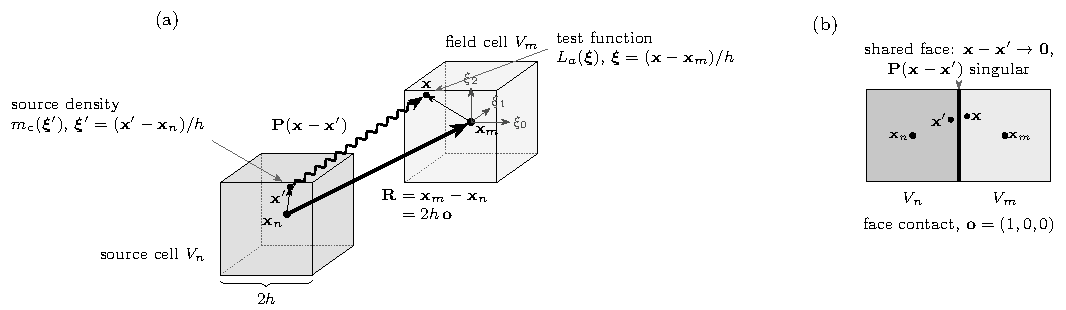
\includegraphics[width=\linewidth]{figures/fig_block.pdf}
\caption{The geometry of the coupling block, Eq.~\eqref{eq:block}. (a) A source cell $V_n$ and a field cell
$V_m$, cubes of side $2h$ with centres $\mathbf x_n$ and $\mathbf x_m$ and integer offset
$\bo=\bR/2h$, here $(2,0,1)$. Each point is located by its cell's local coordinates, $\bxi'$ and
$\bxi$ in $[-1,1]^3$ (the field cell's axes shown). The source density $m_c(\bxi')$ at a source point
$\mathbf x'$ radiates through the point propagator $\bP(\mathbf x-\mathbf x')$ to a field point $\mathbf x$,
where it is weighted by the test function $L_a(\bxi)$; the block is this product integrated over both
cells. (b) A section through two cells in face contact: on the shared face (thick) the field and source
points coincide, so the integrand is singular there. For edge and corner contact the cells share an edge or a
vertex, and the self block has $\mathbf x=\mathbf x'$ throughout the cell.}
\label{fig:block}
\end{figure}

\paragraph{The $s$-form.} With $\mathbf{x}=\mathbf{x}_m+\bu$ and $\mathbf{x}'=\mathbf{x}_n+\bu'$ the kernel
sees $\bR+\bs$, $\bs=\bu-\bu'\in[-2h,2h]^3$, and
\begin{equation}\label{eq:sform}
  \bK_{ac}(\bR)=\int W_{ac}(\bs)\,\bP(\bR+\bs)\,\dd^3s,\qquad W_{ac}(\bs)=\prod_iw_{e_{a,i}e_{c,i}}(s_i),
\end{equation}
with the one-dimensional cross-correlation $w_{\alpha\beta}(s)=h\int v^\alpha(v-s/h)^\beta\,\dd v$ over
$v\in[\max(-1,s/h-1),\min(1,s/h+1)]$. Each factor is a polynomial on $[-2h,0]$ and on $[0,2h]$, continuous,
zero at $\pm2h$, and kinked at $0$ and $\pm2h$. In units of $h$, $\sigma=s/h$, the domain of
Eq.~\eqref{eq:sform} is cut into $8$ boxes on which $W_{ac}$ is a polynomial, whose corners lie on the
breakpoints $\sigma_i\in\{-2,0,2\}$. The kernel is singular at $\bs=-\bR$, that is at
$\boldsymbol\sigma^*=-2\bo$, which for touching cells is always a breakpoint: a vertex of some of the boxes,
and at a distance of at least $2$ (in units of $h$) from the others.

\paragraph{The series in the wavenumber.} With $g_k=\mathrm{e}^{\mathrm{i}kr}/r=\sum_{t\ge0}
(\mathrm{i}k)^tr^{t-1}/t!$, the Green's tensor is a sum over powers $r^m$, $m=t-1\ge-1$, of two families,
\begin{equation}\label{eq:series}
  \bG_{ij}=\frac{1}{4\pi\mu}\sum_{m\ge-1}\Bigl[c_1(m)\,\delta_{ij}\,r^m+c_2(m)\,\partial_i\partial_jr^m\Bigr],
  \qquad c_1=\frac{(\mathrm{i}k_S)^{m+1}}{(m+1)!},\quad
  c_2=\frac{\mathrm{i}^{m+1}\bigl(k_S^{m+1}-k_P^{m+1}\bigr)}{k_S^2\,(m+1)!},
\end{equation}
with $\mu$ the shear modulus and $k_P$, $k_S$ the compressional and shear wavenumbers of the background.
The static (Kelvin) tensor is $c_1$ at $m=-1$ and $c_2$ at $m=1$. Since $\bP$ adds up to two derivatives,
every entry of every block is a combination, with $9\times9$ coefficient tables fixed by the propagator's
structure, of the scalar moments
\begin{equation}\label{eq:umoment}
  \int_{V}\!\int_{V'}L_a(\bxi)\,\partial^{\biota}r^m\,m_c(\bxi')\,\dd^3x\,\dd^3x'
  =h^{\,6+m-|\biota|}\,U_{ac}(m,\biota;\bo),\qquad|\biota|\le4,
\end{equation}
where $\biota$ is the multi-index of derivatives with respect to $\mathbf{x}$. The $U$ are pure numbers:
they depend on neither the frequency, the cell size nor the medium. For even $m$, $r^m$ is a polynomial
and the moment is an integral of polynomials over the boxes, exact by a Gauss rule of sufficient order.
The odd $m$ carry the singularity, and they are the subject of this paper.

\paragraph{Moving derivatives.} For $m=-1$ and $m=1$ with enough derivatives the kernel
$\partial^{\biota} r^m$ is a distribution at the singular point. Of the derivatives in $\biota$,
$k=\max\bigl(0,|\biota|-\min(m+1,\tfrac{m+3}{2})\bigr)\le2$ are moved onto $W$:
$\int W\,\partial^{\biota} f=(-1)^k\int(\partial^{\text{moved}}W)\,\partial^{\text{rest}}f$. What remains,
$\partial^{\text{rest}}r^m$, is at most $1/r$ singular, and it is a sum of monomials times odd powers of
the distance,
\begin{equation}\label{eq:monomials}
  \partial^{\text{rest}}r^m=\sum_j\gamma_j\,\bt^{\balpha_j}\,|\bt|^{n_j},\qquad
  \partial_i\bigl(\bt^{\balpha}|\bt|^n\bigr)=\alpha_i\,\bt^{\balpha-\mathbf{e}_i}|\bt|^n+n\,\bt^{\balpha+
  \mathbf{e}_i}|\bt|^{n-2},
\end{equation}
in the separation $\bt=\boldsymbol\sigma-\boldsymbol\sigma^*$ measured from the singular point, with
$|\balpha_j|+n_j=m-|\text{rest}|$ for every $j$. Two moved derivatives on one axis turn the kinks of $w$
into plane deltas $J_b\,\delta(\sigma-b)$, $b\in\{-2,0,2\}$, $J_b$ the jump of $w'$ at $b$. Each term of a
moment is therefore an integral of a polynomial in $\bt$ times $\bt^{\balpha}|\bt|^n$ over a box of side $2$
whose corners lie on the breakpoints, or over a face of one when a plane delta fixes a coordinate. This is
the object every route below evaluates; they differ only in how.

\subsection{Does the two-centre multipole series work for cells that touch?}\label{sec:twocentre}

\paragraph{The two-centre expansion.} The block \eqref{eq:sform} depends on the two cells only through the
separation $\bR+\bs$ of a field point and a source point. Expanding the propagator about the separation of
the centres, $\bP(\bR+\bs)=\sum_{\boldsymbol\gamma}\bs^{\boldsymbol\gamma}\partial^{\boldsymbol\gamma}\bP(\bR)
/\boldsymbol\gamma!$, and integrating term by term over the two cells gives
\begin{equation}\label{eq:twocentre}
  \bK_{ac}(\bR)=\sum_{\boldsymbol\gamma}\frac{h^{\,6+|\boldsymbol\gamma|}}{\boldsymbol\gamma!}\,
  \mu^{\boldsymbol\gamma}_{ac}\,\partial^{\boldsymbol\gamma}\bP(\bR),\qquad
  \mu^{\boldsymbol\gamma}_{ac}=\int\!\!\int\bxi^{\mathbf e_a}(\bxi-\bxi')^{\boldsymbol\gamma}\,
  \bxi'^{\,\mathbf e_c}\,\dd^3\xi\,\dd^3\xi',
\end{equation}
with the multi-index $\boldsymbol\gamma$ running over all orders. The pair moments
$\mu^{\boldsymbol\gamma}_{ac}$ are products of one-dimensional integrals of monomials, rational numbers, and
the separation enters only through the derivatives of the propagator at one point, which are elementary.
No singular integral appears: the two cells are replaced by their multipole moments about their own
centres (Figure~\ref{fig:twocentre}(a)). Equation~\eqref{eq:twocentre} is the Cartesian counterpart of the
translation addition theorem by which superposition $T$-matrix methods couple scatterers, each represented
about its own origin \citep{MishchenkoTravisLacis2002}, and it is the series used for distant cells in
\S\ref{sec:distant}.

\begin{figure}[t]
\centering
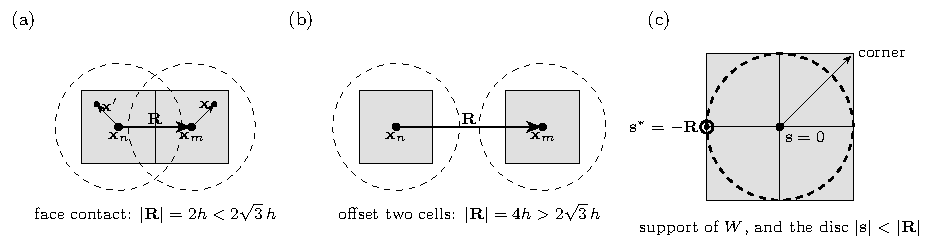
\includegraphics[width=\linewidth]{figures/fig_twocentre.pdf}
\caption{The two-centre expansion, in a section through the cell centres. (a) Two cells in face contact,
centres $\mathbf x_n$ and $\mathbf x_m$ a distance $|\bR|=2h$ apart, with a source point $\mathbf x'$ and a
field point $\mathbf x$; the dashed circles are the sections of the circumscribing spheres, of radius
$\sqrt3\,h$, which overlap. (b) Cells two widths apart, $|\bR|=4h>2\sqrt3\,h$: the spheres are disjoint.
(c) The separation $\bs=(\mathbf x-\mathbf x_m)-(\mathbf x'-\mathbf x_n)$ for face contact: the shaded square
is the support of the pair's cross-correlation $W$ (four of its eight pieces in this section), the dashed
circle the disc
$|\bs|<|\bR|$ on which the Taylor series of $\bP(\bR+\bs)$ about $\bs=0$ converges, and the ringed point the
singular point $\bs^*=-\bR$, on the boundary of the support. The support reaches beyond the disc, to
$|\bs|=2\sqrt3\,h$ at its corners in three dimensions.}
\label{fig:twocentre}
\end{figure}

\paragraph{The condition, and why every neighbour violates it.} The Taylor series of $\bP(\bR+\bs)$ about
$\bs=0$ converges for $|\bs|<|\bR|$, the distance from the expansion point to the singular point
$\bs^*=-\bR$. The separation ranges over the support of $W$, $|s_i|\le2h$, as far as $|\bs|=2\sqrt3\,h$,
the sum of the radii of the two cells' circumscribing spheres. The series is therefore assured to converge
only when $2\sqrt3\,h<|\bR|$, that is when the circumscribing spheres do not overlap
(Figure~\ref{fig:twocentre}(b)). Superposition $T$-matrix methods state the same condition: the smallest
circumscribing spheres of the components must not overlap \citep[\S5.9]{MishchenkoTravisLacis2002}, and
each particle's circumscribing sphere must not intersect its neighbours \citep{TheobaldEgelGomardLemmer2017}.
The condition is sufficient rather than necessary: for adjacent spheroids, results converge well beyond it,
although extreme overlap needed quadruple precision \citep{SchebarchovLeRuGrandAuguie2019}. A space-filling
tessellation violates it for each of a cell's $26$ neighbours (Figure~\ref{fig:neighbours}), with the ratio $\rho=2\sqrt3\,h/|\bR|$ equal
to $\sqrt3$, $\sqrt{3/2}$ and $1$ at face, edge and corner contact, and for touching cells the singular point
lies on the boundary of the support (Figure~\ref{fig:twocentre}(c)). Whether the series converges there
anyway is a question of fact, and it decides whether the closed forms of this paper are needed at all.

\begin{figure}[t]
\centering
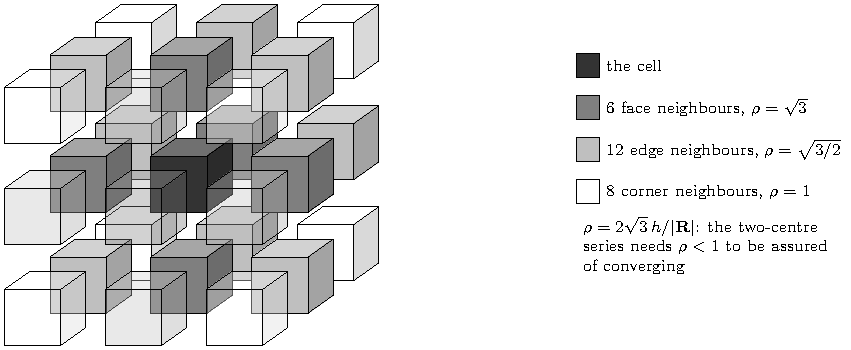
\includegraphics[width=0.92\linewidth]{figures/fig_neighbours.pdf}
\caption{A cell of a space-filling tessellation and its $26$ neighbours, drawn apart so that the cell
(darkest) can be seen, with the nine cubes of the front layer see-through. The neighbours touch it across
a face ($6$), an edge ($12$) or a corner ($8$); for each the ratio $\rho=2\sqrt3\,h/|\mathbf R|$ of the
two circumscribing radii to the distance of the centres is at least one, so none satisfies the condition
under which the two-centre series is assured to converge (Table~\ref{tab:twocentre}).}
\label{fig:neighbours}
\end{figure}

\paragraph{The experiment.} The quantity tested is the coupling moment of the kernel $1/r$,
$U_{ac}(\bo)=\int\!\int\bxi^{\mathbf e_a}\,|\mathbf x-\mathbf x'|^{-1}\,\bxi'^{\,\mathbf e_c}$, for cells
of half-width $h=1$ carrying a linear field (four test monomials and ten source monomials). The kernel
$1/r$ is the static singular part that every family of the propagator shares (the term $m=-1$ of
Eq.~\eqref{eq:series}), so its behaviour is the behaviour of the series for every block. The exact value
is, for cells that touch, the stable closed form of \S\ref{sec:stable}, accurate to round-off against the
forty-digit reference of \S\ref{sec:reference}; for cells apart, Gauss rules of $32$ points per axis on
each of the eight pieces of the $s$-form, which reach round-off because the integrand is then smooth. The
series \eqref{eq:twocentre} is summed in $60$-digit arithmetic, with the pair moments exact as rationals
and the derivatives of $1/r$ at $\bR$ from their Hermite-type expansion with integer coefficients, so that
divergence cannot be mistaken for rounding. The partial sums $S_N$, over all $|\boldsymbol\gamma|\le N$,
are compared with the exact value; the same sums in double precision give the condition number
$\kappa_N=\sum|\text{terms}|/|S_N|$ over the entries larger than $10^{-6}$ of the largest
(\path{scripts/measure_touching_multipole_series.py}).

\begin{table}[h]
\centering
\small
\begin{tabular}{lcccccc}
\toprule
offset $\bo$ & $\rho$ & $N=8$ & $N=16$ & $N=32$ & $N=48$ & $\kappa_{48}$ \\
\midrule
$(1,0,0)$, face   & $1.73$ & $1.0\times10^{-2}$ & $1.5\times10^{-2}$ & $1.5$ & $1.2\times10^{3}$ & $2.2\times10^{12}$ \\
$(1,1,0)$, edge   & $1.22$ & $3.5\times10^{-4}$ & $5.2\times10^{-5}$ & $3.1\times10^{-5}$ & $6.6\times10^{-5}$ & $1.0\times10^{6}$ \\
$(1,1,1)$, corner & $1.00$ & $8.8\times10^{-5}$ & $6.3\times10^{-6}$ & $3.4\times10^{-7}$ & $5.4\times10^{-8}$ & $4.6\times10^{2}$ \\
$(2,0,0)$         & $0.87$ & $1.2\times10^{-5}$ & $1.6\times10^{-7}$ & $3.2\times10^{-10}$ & $2.6\times10^{-12}$ & $3.5$ \\
$(2,1,1)$         & $0.71$ & $2.1\times10^{-6}$ & $4.6\times10^{-9}$ & $3.2\times10^{-13}$ & $7.4\times10^{-16}$ & $6.5$ \\
$(3,0,0)$         & $0.58$ & $3.7\times10^{-7}$ & $1.6\times10^{-10}$ & $1.3\times10^{-15}$ & $1.0\times10^{-15}$ & $1.4$ \\
\bottomrule
\end{tabular}
\caption{The two-centre series \eqref{eq:twocentre} for the kernel $1/r$: error of the partial sum $S_N$,
summed in $60$-digit arithmetic, relative to the largest entry of the exact moment, and the condition
number of the sum in double precision at $N=48$. $\rho=2\sqrt3\,h/|\bR|$ is the ratio of the two
circumscribing radii to the distance of the centres.}
\label{tab:twocentre}
\end{table}

\paragraph{What it shows.} The answer is no (Table~\ref{tab:twocentre}). At face contact the series
diverges: at every fourth order from $0$ to $48$ its error is at least $10^{-2}$, the smallest at $N=4$
and $8$, and from $N=12$ it grows, to $1.2\times10^{3}$ at $N=48$. At edge contact it reaches
$1.3\times10^{-5}$ at $N=24$ and then grows again, to $6.6\times10^{-5}$ at $N=48$, without converging. At corner contact, where
the circumscribing spheres just touch, it converges, but only algebraically, to $5\times10^{-8}$ at $N=48$.
Cells that do not touch converge geometrically, the faster the smaller $\rho$, as the condition predicts;
at the offset $(3,0,0)$ the series reaches round-off by $N=32$. Precision does not change this: at the three touching
geometries the $60$-digit and double-precision sums agree to every digit shown, so the failure is the
series', not the arithmetic's, and the remedy that rescued adjacent spheroids, more digits, does nothing
here. The condition number of the sum tells the same story from the other side: $\kappa_{48}$ is
$2\times10^{12}$ at face contact and of order one for the separated cells.

\paragraph{Subdivision does not rescue it.} For cells that do not touch, the series can be made to converge
faster by cutting the support into boxes and expanding about each box's own centre (\S\ref{sec:distant}).
For cells that touch it cannot: a box whose closure holds the singular point $\bs^*$ has its centre within
one half-diagonal of it, so its own ratio is at least one, however finely the support is cut, and such a box
always exists because $\bs^*$ lies on the boundary of the support. The interaction of a cell with its
neighbours, which in a space-filling medium is where the coupling of the continuum lives, is therefore out
of reach of the expansion that methods leaving gaps between their scatterers rely on. That is the reason
for the closed forms of the rest of this paper.

\section{The closed forms, and why they fail in double precision}\label{sec:failure}

\paragraph{Measuring the loss.} Every evaluation below ends in a sum, $S=\sum_na_n$, of terms computed to
a relative accuracy near the unit round-off $\varepsilon$. Its rounding error is then at most about
$\varepsilon\sum_n|a_n|$, so that the sum loses about $\log_{10}\kappa$ significant digits, with
\begin{equation}\label{eq:kappa}
  \kappa=\frac{\sum_n|a_n|}{\bigl|\sum_na_n\bigr|}
\end{equation}
its condition number \citep{Higham2002}; $\kappa=10^{8}$ leaves about eight good digits in double
precision. An integral has a condition number of its own,
$\kappa_{\mathord{\int}}(f)=\int|f|\,\big/\,\bigl|\int f\bigr|$, and it is the floor below which no method that works from
the values of the integrand can be expected to go. If the integrand is perturbed by $\delta f$ with
$|\delta f|\le\varepsilon|f|$ at every point, then $|\int\delta f|\le\varepsilon\int|f|$, so the relative
change of the integral is at most $\varepsilon\,\kappa_{\mathord{\int}}(f)$, and the perturbation
$\delta f=\varepsilon|f|\operatorname{sgn}\int f$ attains it. A Gauss rule with positive weights computes
$\sum_iw_if(\mathbf x_i)$, whose condition number tends to $\kappa_{\mathord{\int}}(f)$ as the rule converges, because
the same weights integrate $|f|$; quadrature therefore loses about as many digits as the problem itself
forces. A closed form instead writes the integral as a sum of its own choosing, and its condition number
$\kappa$ can be far larger than $\kappa_{\mathord{\int}}$: that excess, and nothing else, is what an evaluation in
closed form has to remove. The rest of this section measures it.

\paragraph{The closed forms as written.} The integrand $\bt^{\balpha}|\bt|^n$ is homogeneous about the
singular point, and three master integrals anchored there are elementary:
\begin{align}
  I[p,q,r;a,b,c;n]&=\int_0^a\!\!\int_0^b\!\!\int_0^c x^py^qz^r\,(x^2+y^2+z^2)^{n/2}\,\dd z\,\dd y\,\dd x,
  \label{eq:boxI}\\
  J[q,r;a;b,c;n]&=\int_0^b\!\!\int_0^c y^qz^r\,(a^2+y^2+z^2)^{n/2}\,\dd z\,\dd y,\label{eq:faceJ}\\
  L[r;A;c;n]&=\int_0^c z^r\,(A^2+z^2)^{n/2}\,\dd z,\label{eq:lineL}
\end{align}
with $n$ odd. Euler's identity for a homogeneous function and the divergence theorem reduce the box to
faces, the faces through the singular point carrying no flux; on a face, the derivative of
$y^{q-1}(a^2+y^2+z^2)^{(n+2)/2}$ lowers the power of $y$ by two and leaves edge integrals; on an edge the
same step ends in a power, a square root or an inverse hyperbolic sine. One transcendental base case is
left on the faces, $J[0,0;a;b,c;-3]=a^{-1}\arctan\bigl(bc/(a\sqrt{a^2+b^2+c^2})\bigr)$, $1/a$ times the
solid angle the rectangle subtends at the singular point. The recursions divide by small integers only,
and they were evaluated at forty digits. To use them for a box that is not anchored at the singular point,
two steps are needed. On each axis an integral from $l$ to $u$ is the difference of two integrals from the
origin (the singular point), so a box at a distance becomes a signed sum of eight anchored boxes of sides
$2$ and $4$. And the polynomial weight is expanded in powers of $\bt$, so that each term is a master
integral. The master integrals, rounded to double precision, were then contracted with the expanded
weights in double precision.

\paragraph{How large the loss is.} Against the forty-digit reference of \S\ref{sec:reference}, the static
coupling block assembled this way is wrong by $2.3\times10^{-13}$ (linear field, corner contact),
$9.4\times10^{-14}$ (linear, edge), $1.7\times10^{-11}$ (quadratic, corner) and $5.5\times10^{-12}$
(quadratic, edge), relative error in the Frobenius norm over all entries of the block. Quadrature of the
same block (Duffy pyramids at the singular vertex and tensor Gauss rules of $20$ points per axis on the
pieces) is accurate to $1.1\times10^{-15}$, $1.8\times10^{-15}$, $1.9\times10^{-15}$ and $2.7\times10^{-15}$.
The closed forms, exact on paper, are worse than quadrature by two orders of magnitude for a linear field
and four for a quadratic one. The loss went unnoticed because the closed forms had been checked against
quadrature to $10^{-9}$ only.

\paragraph{Where it is lost.} Each block is a sum over the pieces of $W$. Taking one term, $m=1$ with
$\biota=(0,2,2)$, at corner contact with a linear field, and evaluating the same algorithm once in double
precision and once with every step at forty digits, the difference piece by piece is $2.1\times10^{-12}$
(relative to the largest entry of the term) on the piece farthest from the singular point, the box
$\bt\in[2,4]^3$, and at most $1.2\times10^{-15}$ on the piece that has the singular point as a vertex.
The loss is in the pieces away from the singular point.

\paragraph{Why it is lost.} On such a piece two cancellations act together: the inclusion-exclusion of
anchored boxes, and the power basis about a point outside the piece. They can be separated. On the far
piece of the corner contact, for the same term, the integral was computed four ways, each compared with
the same piece at forty digits with exact rational weights:
\begin{itemize}
  \item[A] as written: anchored master integrals rounded to double precision, inclusion-exclusion and
  contraction in double precision. Error $2.6\times10^{-13}$.
  \item[B] the moments of the far box itself, $\int_{\text{box}}\bt^{\mathbf{e}}|\bt|^n$, exact
  (inclusion-exclusion at forty digits) and then rounded; the contraction with the power-basis weights in
  double precision. Error $6.7\times10^{-14}$.
  \item[C] as B, with the contraction at forty digits too, the weights still rounded to double
  precision. Error $8.6\times10^{-15}$.
  \item[D] the weight re-expanded about the piece's own corner, in the local variable
  $\boldsymbol\tau=\bt-\mathbf{l}\in[0,2]^3$, with the local moments $\int\boldsymbol\tau^{\mathbf{j}}
  \bt^{\balpha}|\bt|^n$ exact and rounded, and a double-precision contraction. Error $6.8\times10^{-16}$.
\end{itemize}
Inclusion-exclusion accounts for a factor of four (A against B). The rest is the power basis about the
singular point: the moments reach $2\times10^{19}$ against a piece of order one, so that the rounding of
the weights alone (C) costs three digits. A basis local to the piece removes the loss entirely (D). At
quadratic degree the local power basis is itself not quite enough: with exact moments the far piece is
accurate to $4.9\times10^{-15}$ in local powers and to $1.9\times10^{-16}$ in Legendre polynomials of the
local coordinate, and the piece at the singular point to $4.0\times10^{-15}$ and $2.4\times10^{-16}$. The
basis the evaluation needs is therefore the Legendre basis of each piece. This is the classical
conditioning contrast between power moments and orthogonal-polynomial (modified) moments
\citep{Gautschi1970}.

\paragraph{Quadrature on the smooth pieces is not enough.} A natural alternative keeps the closed forms only
on the pieces that hold the singular point and integrates the others, which are smooth, by Gauss rules.
It cures the linear field ($9.1\times10^{-16}$ and $1.6\times10^{-15}$ at corner and edge) but not the
quadratic one ($5.9\times10^{-15}$ and $1.1\times10^{-14}$, insensitive to the Gauss order between $12$ and
$20$), because at quadratic degree the pieces at the singular point lose digits too, to the power basis
on $[0,2]$. The same switch is the remedy adopted for analytic boundary-element integrals
\citep{KanekoGumerovDuraiswami2024,GumerovKanekoDuraiswami2024}; here it does not reach round-off, and
it gives up the frequency-independent coefficients only on part of the domain while keeping the
ill-conditioned basis on the rest.

\section{A forty-digit reference}\label{sec:reference}

A reference must share no step with the routes it judges. For corner and edge contact one exists that is
also simple. There the singular point is a vertex of the pieces it touches, and $W_{ac}$ vanishes there as
$\rho^3$ (corner) or $\rho^2$ (edge), $\rho$ the distance from the singular point. The most singular static
term, $\partial^4r\sim\rho^{-3}$, is then absolutely integrable, and so is every other: the block is an
ordinary integral, with no distribution, no moved derivative and no master integral.
\texttt{Mathematica/GradedVoxel\_CornerReference.wl} evaluates
\begin{equation}\label{eq:reference}
  \int_{[-2,2]^3}W_{ac}(\bs)\,\partial^{\biota} r^m(\bR+\bs)\,\dd^3s
\end{equation}
for each of the $41$ static terms ($m=-1$ and $m=1$) at forty digits, at $h=1$. The factors of $W_{ac}$
are integrated exactly from their definition. The domain is cut into its $8$ pieces; on a piece with the
singular point at a vertex, three Duffy pyramids \citep{Duffy1982} about that vertex make the integrand
$u_1^{\,k}$ times a smooth function, with $k\ge0$ an integer, so a tensor Gauss rule converges
exponentially; the other pieces are smooth. The terms are assembled into the static block with exact
rational weights and the medium's constants in exact arithmetic. Three gates check it.
\begin{itemize}
  \item[(a)] A polynomial kernel, $|\bR+\bs|^2$, for which Mathematica gives the six-dimensional integral
  of Eq.~\eqref{eq:block} exactly. The reference reproduces it to $10^{-35}$, which checks $W$, the
  pieces, the Duffy map and the weights.
  \item[(b)] Integration by parts on the hardest term: with $F=\partial_0\partial_0\partial_1r$,
  $\int W\,\partial_2F=-\int(\partial_2W)\,F$, the boundary terms vanishing because $W$ is continuous and
  zero on the boundary of its support. The two sides have different integrands and agree only if the
  singular integration is accurate. They agree to $1.4\times10^{-24}$ (corner) and $2.4\times10^{-24}$
  (edge) for the linear field and $3.9\times10^{-24}$ and $3.5\times10^{-24}$ for the quadratic one.
  \item[(c)] Convergence: the rule at $20$ and at $28$ points per axis agree to better than
  $10^{-23}$ in every case ($3\times10^{-25}$ to $2\times10^{-24}$ where the value was recorded). Each piece
  converges by about five digits per four points.
\end{itemize}
Pointwise identities such as $\nabla^2(1/r)=0$, which hold at every node of the rule, would pass whatever
the integration did, and are not used as gates. The reference took $78$ to $93$\,s per geometry for the
linear field and $502$ to $593$\,s for the quadratic one, at $20$ points per axis.

\section{A stable evaluation}\label{sec:stable}

\subsection{Marching the recurrences}\label{sec:marching}

The reductions of \S\ref{sec:failure} can be re-anchored at the corner of each piece, so that the
weights are local. In one dimension the edge moments $E[r]=\int_l^{l+L}u^r(A^2+t^2)^{n/2}\dd t$, with
$t=u+l$, satisfy at fixed $n$ the three-term recurrence
\begin{equation}\label{eq:edgerec}
  (r+n+2)\,E[r+1]+l\,(2r+n+2)\,E[r]+r\,(A^2+l^2)\,E[r-1]=\bigl[u^r(A^2+t^2)^{(n+2)/2}\bigr]_{t=l}^{t=l+L},
\end{equation}
from $\frac{\dd}{\dd t}\bigl(u^r(A^2+t^2)^{(n+2)/2}\bigr)$ with $(A^2+t^2)=(A^2+l^2)+2lu+u^2$. Its homogeneous
solutions grow like $\rho^r$, with $\rho=\sqrt{A^2+l^2}$ the distance from the singular point to the near
end of the edge, while the wanted moments grow like $L^r$. Away from the singular point ($\rho>L$) the
wanted solution is the minimal one, forward recursion amplifies the rounding errors, and backward
recursion from zero values at a high degree converges to it, the error falling like $(L/\rho)^{R-r}$
\citep{Gautschi1967,Olver1967}. Measured against forty-digit quadrature, forward recursion loses up to
$10^{-7}$ by degree $20$ when $\rho/L=2.45$, and backward recursion is at round-off ($2\times10^{-16}$) for
every $\rho/L$ tested, from $1.41$ to $2.45$, including $n=-3$, where the forward recursion fails at once on a zero
divisor. Backward recursion needs no transcendental starting value, only the end terms of
Eq.~\eqref{eq:edgerec}. For $\rho\le L$, near the singular point, forward recursion is the stable direction.

In two dimensions the same identity along one axis acquires cross terms in the other, since
$(c^2+t_y^2+t_z^2)$ involves both, and running it backwards requires a back-substitution in the other index
at every level. This works to round-off (at most $10^{-15}$) on every face tested whose near corner is at
least $1.73$ side lengths from the singular point, but it diverges, to errors of $10^2$ to $10^{97}$, on the
faces at $\sqrt2$ side lengths; forward recursion there reaches only $10^{-9}$ to $2\times10^{-8}$ at
degree $8$, and $4\times10^{-13}$ to $3\times10^{-11}$ at a distance of one side length. There is a band of
geometries next to the singular point in which neither direction is stable, and the faces of the pieces
adjacent to the singular point fall in it. Marching does not give a complete scheme.

\subsection{Legendre moments by a boundary-value relation}\label{sec:legendre}

On the unit box $\prod_j[l_j,l_j+1]$ in $d=1$, $2$ or $3$ dimensions, lifted by $c^2\ge0$ so that
$S^2=c^2+\sum_jt_j^2$, define the Legendre moments
\begin{equation}\label{eq:lam}
  \Lambda[\mathbf{k}]=\int_{\text{box}}\prod_jP_{k_j}(x_j)\,S^m\,\dd^dt,\qquad x_j=2(t_j-l_j)-1\in[-1,1],
\end{equation}
for boxes whose closure does not hold the singular point ($S>0$ on the box). Along an anchor axis $i$, the
Legendre identity $(2k+1)P_k=P'_{k+1}-P'_{k-1}$ and an integration by parts in $x_i$, applied to
$g=S^{m+2}=(c^2+\sum_jt_j^2)\,S^m$, whose derivative is $\partial g/\partial x_i=\frac{m+2}{2}\,t_iS^m$, give
\begin{equation}\label{eq:relation}
  (2k_i+1)\int P_{\mathbf{k}}\Bigl(c^2+\sum_jt_j^2\Bigr)S^m
  +\frac{m+2}{2}\int\bigl(P_{k_i+1}-P_{k_i-1}\bigr)(x_i)\,t_i\,P_{\hat{\mathbf{k}}}\,S^m=0,\qquad k_i\ge1,
\end{equation}
where $P_{\mathbf{k}}=\prod_jP_{k_j}(x_j)$ and $\hat{\mathbf{k}}$ collects the other axes. The boundary
terms vanish because $P_{k_i+1}-P_{k_i-1}$ is zero at $x_i=\pm1$. For $k_i=0$, with $P_0=P_1'$,
\begin{equation}\label{eq:relation0}
  \int P_{\mathbf{k}}\Bigl(c^2+\sum_jt_j^2\Bigr)S^m+\frac{m+2}{2}\int P_1(x_i)\,t_i\,P_{\hat{\mathbf{k}}}\,S^m
  =\tfrac12\Bigl(\Lambda_{d-1}\bigl[\hat{\mathbf{k}};c^2+(l_i+1)^2\bigr]+\Lambda_{d-1}\bigl[\hat{\mathbf{k}};
  c^2+l_i^2\bigr]\Bigr),
\end{equation}
the right side being the moments of $S^{m+2}$ on the two faces normal to axis $i$, one dimension down,
computed by the same relation. In zero dimensions the moment is the corner value $c^{m+2}$. Because
$t_j=l_j+\tfrac12+\tfrac12x_j$, multiplication by $t_j$ and by $t_j^2$ is a banded operator on the
Legendre index (three-term and five-term), so each relation couples $\Lambda$ at the indices $k_j-2$ to
$k_j+2$ in every axis.

\paragraph{The solution.} The anchor is taken as the axis of the largest $k_i$. The relations for
$\mathbf{k}\in[0,N)^d$, with $\Lambda=0$ beyond, form one sparse linear system for the $N^d$ unknowns:
the boundary-value formulation of a recurrence whose wanted solution is the minimal one, solved directly
rather than marched \citep{Olver1967,OlverSookne1972}. The only data are the corner values of $S^{m+2}$
and its analogues one and two dimensions down; no logarithm, inverse hyperbolic sine or arctangent is
evaluated, the transcendental functions being carried by the system. Against forty-digit quadrature the
edge moments come out to full relative accuracy, the high-order ones included: for $k\le16$ the absolute
errors relative to $\Lambda[0]$ are $10^{-20}$ to $10^{-35}$ while the moments themselves fall to
$10^{-13}$ to $10^{-21}$ of $\Lambda[0]$, at $\rho=1$, $\sqrt2$, $\sqrt3$, $\sqrt6$ and $3$ and for
$m=-3$, $-1$ and $1$. The face moments are accurate to $9\times10^{-18}$ to $3\times10^{-16}$ relative to
$\Lambda[0,0]$, including the faces at $\rho=\sqrt2$ and $\rho=1$ where marching failed. The truncation
margin used in these tests is $16$ Legendre degrees beyond the highest needed; in the coupling blocks
$8$ suffices (\S\ref{sec:results}).

\subsection{Pieces away from the singular point}\label{sec:far}

In $\bt$, a piece of $W$ away from the singular point is a box of side $2$ in one orthant (each axis
interval is $[0,2]$, $[2,4]$ or their reflections), or a face of one at $|t_i|=|b-\sigma_i^*|$ for a plane
delta. Reflecting each axis to $t_j\ge0$ and scaling by $\bt=2\tilde{\bt}$ makes it the unit box of
\S\ref{sec:legendre}, with $c^2=(t_i/2)^2$ for a plane delta and $c=0$ otherwise. On each free axis the
weight $w_j(\sigma_j)$ is written as a Legendre series in the box's own coordinate $x_j$; the kernel
monomial $\tilde t_j^{\,\alpha_j}$ multiplies that series in the Legendre basis exactly; and the piece is the
contraction
\begin{equation}\label{eq:farpiece}
  \int_{\text{piece}}W\,\bt^{\balpha}|\bt|^n=2^{\,n+|\balpha|+d}\,\prod_j(\pm1)^{\alpha_j}\sum_{\mathbf{k}}
  \Bigl(\prod_j\bigl[\tilde t_j^{\,\alpha_j}w_j\bigr]_{k_j}\Bigr)\,\Lambda[\mathbf{k}],
\end{equation}
with the fixed coordinates' factors (the jump of $w'$ and $t_i^{\alpha_i}$) in front. The Legendre
coefficients of the weights and the moments are of order one or smaller, and the moments decay with
their degree, so the contraction has no large terms to cancel.

\subsection{Pieces at the singular point}\label{sec:pyramids}

A piece whose closure holds the singular point is, reflected and scaled, $[0,1]^d$ with a corner at the
singular point ($d=3$, or $d=2$ for a plane-delta face through it). Its moments do not exist in the form
\eqref{eq:lam}: the moments of $S^{-3}$ alone diverge at the corner, logarithmically in three dimensions,
although the integrand the kernel actually presents, $\bt^{\balpha}|\bt|^{-3}$ with $|\balpha|=2$, is
integrable; the separate moments do not see the factor $\bt^{\balpha}$. The piece is split instead into $d$ Duffy pyramids about the singular corner.
In pyramid $k$, $\tilde t_k=\varrho$ and $\tilde t_j=\varrho v_j$ for the other axes, $\bv\in[0,1]^{d-1}$,
so $\dd^d\tilde t=\varrho^{d-1}\dd\varrho\,\dd^{d-1}v$ and $|\tilde{\bt}|^n=\varrho^n(1+|\bv|^2)^{n/2}$, and
\begin{equation}\label{eq:pyramid}
  \int_{[0,1]^d}P(\tilde{\bt})\,|\tilde{\bt}|^n\,\dd^d\tilde t
  =\sum_k\int_{[0,1]^{d-1}}(1+|\bv|^2)^{n/2}\,G_k(\bv)\,\dd^{d-1}v,\qquad
  G_k(\bv)=\sum_p\frac{c_p(\bv)}{p+n+d},
\end{equation}
where $P$ is the weight times the kernel monomial and $c_p(\bv)$ is the coefficient of $\varrho^p$ in
$P(\varrho\,\mathbf{e}_k(\bv))$. The radial integral is exact. The coefficients that vanish because $W$
vanishes at the vertex, to order $1-n_{\text{der}}$ on an axis where the vertex is an outer end of the
piece ($\sigma=\pm2$) with $n_{\text{der}}$ derivatives moved onto that axis, and to order zero where it is
the inner breakpoint $\sigma=0$, are set exactly to zero, so that $p+n+d>0$ wherever $c_p\ne0$; a non-zero
coefficient with $p+n+d\le0$ would be a divergent integral and is reported as an error. $G_k$ is a
polynomial on the far face of the pyramid, at unit distance from the singular point. It is projected onto
Legendre polynomials on $[0,1]^{d-1}$ by a Gauss rule exact for its degree ($24$ points per axis, $16$
coefficients), which here only manipulates polynomials and never integrates the singular kernel, and
contracted with the face moments $\Lambda$ of $(1+|\bv|^2)^{n/2}$ from \S\ref{sec:legendre}, with $c^2=1$
and $\mathbf{l}=0$.

\section{Accuracy and cost}\label{sec:results}

\paragraph{Blocks against the reference.} With pieces away from the singular point by
Eq.~\eqref{eq:farpiece} and pieces at it by Eq.~\eqref{eq:pyramid}, the static blocks agree with the
reference as follows (relative Frobenius error, implementation
\path{cubic_scattering/graded_voxel/blocks.static_term_integral_closed}):

\begin{table}[h]
\centering
\small
\begin{tabular}{lcccc}
\toprule
 & linear, corner & linear, edge & quadratic, corner & quadratic, edge \\
\midrule
closed forms as written (\S\ref{sec:failure}) & $2.3\times10^{-13}$ & $9.4\times10^{-14}$ & $1.7\times10^{-11}$ & $5.5\times10^{-12}$\\
stable evaluation (\S\ref{sec:stable}) & $1.0\times10^{-15}$ & $9.7\times10^{-16}$ & $3.7\times10^{-15}$ & $4.3\times10^{-15}$\\
quadrature, $20$ points & $1.1\times10^{-15}$ & $1.8\times10^{-15}$ & $1.9\times10^{-15}$ & $2.7\times10^{-15}$\\
\bottomrule
\end{tabular}
\caption{The static coupling block against the forty-digit reference. A linear field has $4$ test
functions and $10$ source monomials, a quadratic one $10$ and $35$; each block has $81$ entries per pair.}
\label{tab:accuracy}
\end{table}

The remaining gap to quadrature for the quadratic field, a factor of $1.3$ to $1.6$, is round-off, not a
residual defect. Term by term, quadrature's own worst moments are in error by $2$ to $3\times10^{-14}$
relative to the largest entry of the term and the stable evaluation's by about $5\times10^{-14}$, with a
median of about $10^{-15}$ for both. Forming the weights' power coefficients in exact rational arithmetic
before rounding gains only $15$ to $20\%$.

\paragraph{Self and face contact.} The reference does not cover self and face contact, where the static
terms are distributions. There the stable evaluation is compared with quadrature, which the reference
shows to be accurate at corner and edge contact. At $h=1.25$, for all $41$ static terms and all pairs of
the linear field, the two agree to a worst term of $4.2\times10^{-15}$ (self), $9.9\times10^{-15}$ (face),
$3.3\times10^{-14}$ (edge) and $1.8\times10^{-14}$ (corner), with medians of $1.0$ to $1.7\times10^{-15}$.
These comparisons are made at $h\ne1$ on purpose: they also check the physical scaling of each piece by
powers of $h$, which a reference at $h=1$ cannot see.

\paragraph{The complete blocks.} With the dynamic terms of the series \eqref{eq:series} added, the
whole touching block, static and dynamic, is the series summed term by term, each term a universal moment
times $h^{\,6+m-|\biota|}$ and the weights $c_1$, $c_2$. At $k_Sh=0.0625$ it agrees with the quadrature
block at $20$ points per axis to about $10^{-15}$ for the linear field at all four contact geometries, and
to $2$ to $4\times10^{-15}$ for the quadratic field; with the closed forms as written the quadratic field's
blocks had stalled at $9\times10^{-15}$ to $2\times10^{-11}$ (\path{scripts/measure_galerkin_near_blocks.py}).

\paragraph{Cost.} The universal moments are computed once for each contact geometry and cell degree: they
depend on neither the frequency nor the cell size. For all four geometries and both degrees, with the
series carried to the powers that $k_Sh=0.0625$ needs, that one-off step took $3745$\,s on one machine,
against $998$\,s for the closed forms as written: about $0.75$\,s per term against $0.3$\,s, over some
$2600$ terms. Stability has a price, and it is paid once. Each block thereafter costs the assembly of the
series alone, $5$\,ms for the linear field and $33$\,ms for the quadratic one, against $0.4$ to $13$\,s for
a quadrature block at the number of points (14 to 20 per axis) that reaches $10^{-15}$. One frequency
needs all eight blocks: $17.4$\,s by quadrature at $14$ points ($2.3$\,s for the linear field, $15.1$\,s
for the quadratic), $0.15$\,s by the series. The one-off cost is therefore recovered after about $220$
frequencies, and a synthetic over $256$ frequencies is already cheaper by the series
(\S\ref{sec:sweep}). Two measures brought the one-off cost down by a factor of $2.3$ without
changing any block beyond round-off: a truncation margin of $8$ Legendre degrees instead of $16$ (the blocks
are the same to the digits shown for margins from $4$ to $16$), and one truncation shared by every term
of a cell degree, so that the sparse systems are solved once and reused.

\section{Multipoles for elastic waves}\label{sec:multipoles}

The word multipole is used in two senses in what follows, and the difference matters. In the first, a
source is resolved into its Cartesian moments while the Green's tensor is integrated exactly: the
Cartesian multipole hierarchy of \citet{NestorContinuum2026}, whose cell-to-cell tables
(\S\ref{sec:sweep}) are exact at every separation. In the second, the usual one, the kernel itself is
expanded about a centre and truncated, which converges only when the cells are far enough apart: the
series for distant cells of \S\ref{sec:distant}. The second is what the fast multipole method rests on
\citep{CarrierGreengardRokhlin1988}; four things make it different for elastic waves and polynomial cubes.

\paragraph{Two wave speeds.} The Green's tensor \eqref{eq:series} is a shear term plus the gradient of a
difference of a shear and a compressional term divided by $k_S^2$ \citep{WuAki1985}, and that difference is finite at
small distance only by cancellation. No single addition theorem serves, and the cancellation has to be
removed analytically rather than numerically: evaluated as the difference of the two spherical-Hankel
forms, the derivatives of $(g_S-g_P)/k_S^2$ lose accuracy as $\varepsilon/(kR)^2$, $\varepsilon$ the
machine precision. Measured, the blocks of cells $3$ to $64$ cells apart at $k_Sh=10^{-4}$ were wrong by
$3\times10^{-9}$ to $10^{-12}$, as that law predicts; with the derivatives taken from the power series of
the difference for $k_Sr\le1$, they are accurate to $10^{-15}$ to $8\times10^{-15}$.

\paragraph{A nine-component state.} The state carries an independent strain, so the propagator $\bP$
carries up to two more derivatives than the Green's tensor, and the sources are forces and stresses
rather than charges. The derivatives of every order are combinations of the radial functions
$F_q=(r^{-1}\dd/\dd r)^q f$ of two scalars, $g_S$ and $(g_S-g_P)/k_S^2$, through fixed tables.

\paragraph{Cubes carrying polynomials.} The natural multipoles are not spherical moments of a point
source but Cartesian moments of two cells at once,
$\mu^{\boldsymbol\gamma}_{ac}=\int\!\!\int\bxi^{\mathbf e_a}(\bxi-\bxi')^{\boldsymbol\gamma}\bxi'^{\,\mathbf e_c}
\dd\bxi\,\dd\bxi'$, products of one-dimensional integrals of monomials, rational numbers.

\paragraph{The radius of convergence.} The separation $\bs$ of two points of the cells ranges over
$|\bs|\le2\sqrt3\,h$, so the expansion about the centre separation $\bR$ converges geometrically in
$\rho=2\sqrt3\,h/R$, the extent of both cells over their distance, and the wavenumber enters only through
the derivatives at $\bR$: the term of order $n$ is bounded by $\sum_j\rho^{\,n-j}\kappa^j/j!$ with
$\kappa=2\sqrt3\,k_Sh$. There is no restriction on $k_SR$, but the series needs $\rho<1$.

\section{Distant cells}\label{sec:distant}

For two cells that do not touch, the kernel is analytic over the whole range of the separation $\bs$,
and the block \eqref{eq:block} can be had without quadrature as the two-centre series
\eqref{eq:twocentre} of \S\ref{sec:twocentre}, which converges when the circumscribing spheres of the two
cells do not overlap, with the two cells' moments $\mu^{\boldsymbol\gamma}_{ac}$ of \S\ref{sec:multipoles} and the derivatives
of the propagator at $\bR$ from those of the two radial scalars. The derivatives of $g_k$ are spherical
Hankel functions, $F_q=\mathrm{i}(-1)^qk^{q+1}h_q(kr)/r^q$; those of $(g_S-g_P)/k_S^2$ come from its power
series for $k_Sr\le1$ and from the difference of the two Hankel forms beyond
(\S\ref{sec:multipoles}). The series converges geometrically in $\rho=2\sqrt3\,h/R$ and is refused for
$\rho>0.6$, about three cells apart; it is truncated at the order where the bound of
\S\ref{sec:multipoles} falls below the tolerance (\path{multipole.far_block_multipole}).

\paragraph{Every pair that does not touch.} Close to contact the series about the cell centres converges
too slowly: at two cells apart $\rho=0.87$. The cross-correlation $W_{ac}$ is a polynomial on each of the
eight boxes of its support, so each box can be expanded about its own centre $\bs_B$, the moments being
those of a polynomial over a box, exact, and the ratio becoming the box's half-diagonal over
$|\bR+\bs_B|$: $0.52$ at two cells apart, and $0.33$ after one bisection of the boxes, each bisection
halving it (\path{multipole.piecewise_multipole_block}). The order is chosen with the bisection level to
minimise the cost, subject to one constraint found by measurement: at the offset $(2,1,1)$ a plan of
order $48$ to $56$ without bisection stalled at $6\times10^{-13}$ to $2\times10^{-12}$, while one bisection
at order $36$ to $40$ reached $10^{-15}$ to $4\times10^{-15}$. The rounding of a series that long grows
with its order, so the order is capped at $40$ and a plan that needs more bisects instead.

\paragraph{The experiment.} For a linear field, at offsets from two to sixty-four cells and at
$k_Sh=10^{-4}$, $0.0625$, $0.5$ and $2$, every route was compared with the $s$-form integrated by Gauss
rules of $32$ points per axis on each of its eight pieces; that reference agrees with $24$ points to
$2\times10^{-15}$ (to $10^{-14}$ at $k_Sh=2$). Four routes were timed per block, warm, the one-off
moments and coefficients excluded: the $s$-form with the package's Gauss rule, the series
\eqref{eq:twocentre}, its piecewise form, and the frequency-independent series in $k$ of
\S\ref{sec:sweep} (\path{scripts/measure_distant_cell_blocks.py}).

\paragraph{Accuracy.} After the corrections below, every route is at round-off wherever it applies: the
largest relative error over all offsets and frequencies is $9\times10^{-15}$ for the Gauss rule and
$10^{-14}$ for the two multipole forms, the same as the reference's own agreement between $24$ and $32$
points. The series in $k$ is at round-off where it converges, and loses accuracy as $k_Sr$ grows,
$5\times10^{-13}$ at sixty-four cells for $k_Sh=0.0625$, because its terms grow like $(k_Sr)^t/t!$ before
they fall; beyond about $k_Sr=14$ it refuses. Two defects were found and corrected by this experiment.
The first is the cancellation of \S\ref{sec:multipoles}: with the derivatives of $(g_S-g_P)/k_S^2$ taken
as a difference of Hankel forms, the multipole blocks at $k_Sh=10^{-4}$ were wrong by $3\times10^{-9}$ to
$10^{-12}$, and the piecewise form near contact by up to $9\times10^{-5}$. The second is in the Gauss rule
itself: its order had been chosen by distance alone, eight points per axis beyond four cells, which
leaves the blocks wrong by $3\times10^{-11}$ at $k_Sh=2$ and by $10^{-6}$ at $k_Sh=4$. Measured against
forty points, the order that reaches about $10^{-14}$ is the larger of the distance rule and
$8+2\lceil k_Sh-1\rceil$, for offsets from two to thirty-two cells and $k_Sh$ up to $4$.

\begin{table}[h]
\centering
\small
\begin{tabular}{rcccc}
\toprule
offset & Gauss & multipole series & piecewise series & series in $k$ \\
\midrule
$(2,0,0)$ & $28$\,ms & refused & $15.8$\,s & $0.8$\,ms \\
$(2,1,1)$ & $26$\,ms & refused & $15.7$\,s & $0.8$\,ms \\
$(3,0,0)$ & $13$\,ms & $9.6$\,s & $2.2$\,s & $0.9$\,ms \\
$(4,3,2)$ & $12$\,ms & $0.62$\,s & $0.73$\,s & $1.1$\,ms \\
$(8,0,0)$ & $8$\,ms & $0.29$\,s & $0.49$\,s & refused \\
$(64,0,0)$ & $8$\,ms & $0.12$\,s & $0.38$\,s & refused \\
\bottomrule
\end{tabular}
\caption{Cost per block for a linear field at $k_Sh=0.5$, every route accurate to round-off. At
$k_Sh=2$ the Gauss rule costs $11$ to $32$\,ms, the two multipole forms $1.5$ to $50$\,s, and the series
in $k$ is refused at every offset; at $k_Sh=10^{-4}$ the multipole series falls to $15$\,ms at sixty-four
cells.}
\label{tab:distant}
\end{table}

\paragraph{What the routes are for.} On a regular grid the distant blocks are needed once per offset
orbit and frequency, and the Gauss rule of the $s$-form, with its order now tied to the frequency, is the
practical route: it is accurate to round-off at every separation and frequency tested, at $8$ to
$32$\,ms a block. The series in $k$ is faster still, under a millisecond a block, wherever $k_Sr$ is
small enough for it, which is the touching and near cells of a sweep at low frequency
(\S\ref{sec:sweep}). The multipole series is the slowest, by one to four orders of magnitude, and it has
one property the others lack: it is exact term by term, with no restriction on $k_SR$, so it is the
independent check of the other two, and it is the form a fast multipole method would use for cells far
apart (\S\ref{sec:fmm}).

\paragraph{A quadratic field.} The same comparison for a quadratic field ($10$ test functions, $35$
source monomials), at offsets $(2,0,0)$, $(2,1,1)$, $(4,3,2)$ and $(16,0,0)$ and at $k_Sh=10^{-4}$,
$0.5$ and $2$, puts every route at round-off again: the largest error is $2\times10^{-14}$, the Gauss
rule at sixteen cells and $k_Sh=2$. The costs rise with the block: $25$ to $93$\,ms for the Gauss rule,
$53$\,ms to $3.1$\,s for the multipole series, $1$ to $172$\,s for its piecewise form, and $1.8$ to
$5.5$\,ms for the series in $k$ where it converges. The ranking of the routes is unchanged.

\section{Frequency-independent coefficients, and the frequency sweep}\label{sec:sweep}

A synthetic seismogram needs the coupling blocks at every frequency of a sweep, at least $256$ of them.
What can be computed once, for the geometry alone, and what must be computed again at each frequency,
decides the cost. The universal moments of the touching blocks are of the first kind. The same structure
serves the blocks between cells that do not touch, and the cell-to-cell tables of the Cartesian multipole hierarchy of
\citet{NestorContinuum2026}, whose integrals are never singular (the field point is a cell centre, at least
half a cell outside the source cube).

\paragraph{The series for cells that do not touch.} For two cells that do not touch, the kernel is smooth
on every piece of $W$, and the series \eqref{eq:series} applies term by term with coefficients obtained by
a Gauss rule on the unit cell, once for each offset:
\begin{equation}\label{eq:farseries}
  \bK_{ac}(\bR)=\sum_{t\ge0}\Bigl[c_1(t-1)\,\mathbf{S}^A_{ac}(t;h)+c_2(t-1)\,\mathbf{S}^B_{ac}(t;h)\Bigr],
  \qquad\mathbf{S}(t;h)=h^{\,6+(t-1)-|\mathbf{a}|}\,\mathbf{S}(t;1),
\end{equation}
where $\mathbf{S}^A$ and $\mathbf{S}^B$ are the $s$-form integrals \eqref{eq:sform} of the propagator built
from $\delta_{ij}r^{t-1}$ and from $\partial_i\partial_jr^{t-1}$, and $|\mathbf{a}|$ is the number of
derivatives on $r^{t-1}$ in each of the $81$ entries (two more for the second family). Because quadrature is
linear in the kernel, the series summed with these coefficients equals the Gauss block exactly, up to the
truncation of the series. It agrees with the Gauss block to $10^{-15}$ to $10^{-13}$ for offsets from two
to five cells and $k_Sh$ from $10^{-6}$ to $0.5$, and costs $0.3$\,ms per block and frequency against
$9$\,ms for the Gauss block (\path{blocks.far_block_series}).

\paragraph{The hierarchy's tables.} The Cartesian multipole hierarchy couples cells through the tables
\begin{equation}\label{eq:hiertable}
  T_{in}[\mathbf{D},\mathbf{W}](\bo)=\int_{\text{cube}}\partial^{\mathbf{D}}\bG_{in}(\bo-\bxi)\,
  \bxi^{\mathbf{W}}\,\dd^3\xi,
\end{equation}
the derivatives of the Green's tensor at the field cell's centre against the source cube's monomials. The
same expansion gives
\begin{equation}\label{eq:hierseries}
  T_{in}[\mathbf{D},\mathbf{W}]=\frac{1}{4\pi\mu}\sum_{t\ge0}\Bigl[c_1(t)\,\delta_{in}\,
  U(t;\mathbf{D},\mathbf{W})+c_2(t)\,U(t;\mathbf{D}+\mathbf{e}_i+\mathbf{e}_n,\mathbf{W})\Bigr],
\end{equation}
now with $c_1(t)=(\mathrm{i}k_S)^t/t!$ and $c_2(t)=((\mathrm{i}k_S)^t-(\mathrm{i}k_P)^t)/(t!\,k_S^2)$, and
$U(t;\mathbf{a},\mathbf{W})=\int\partial^{\mathbf{a}}r^{t-1}(\bo-\bxi)\,\bxi^{\mathbf{W}}\dd^3\xi$ on the
unit cube, scaled to a cube of side $d$ by $d^{\,(t-1)-|\mathbf{a}|+|\mathbf{W}|+3}$. The $U$ are computed
once per offset by a Gauss rule chosen by the offset's shape: $28$ points per axis for a face neighbour,
$20$ for an edge neighbour, $14$ for a corner neighbour and $12$ beyond, each measured to reach $10^{-14}$
against $36$ points for every derivative and weight of the third-gradient hierarchy. Each frequency then
costs one weighted sum. The series agrees with Gauss quadrature at $36$ points to $10^{-15}$ to
$6\times10^{-14}$ from $k_Sd=10^{-6}$ to $3$ (\path{derivatives.moment_table_kseries}); at $48$ terms
it covers $k_S r$ up to about $14$, $r$ the largest distance from the field point to the source cube, and
beyond that it refuses, with the Gauss table as the route.

\paragraph{The stopping rule.} The weight $c_2$ carries $k_S^{-2}$: its term $t$ is of order $k^{t-2}$, as
large as the $c_1$ term $t-2$, and the radiation (imaginary) part at order $k$ comes from $t=1$ of the first
family and $t=3$ of the second together. Each series is therefore summed through $t=4$ at least, and until
$(k_Sr_{\max})^{t-2}/(t-2)!$ falls below the tolerance, $r_{\max}$ the largest separation of two points of
the cells. A rule that bounded term $t$ by $(k_Sr_{\max})^t/t!$, ignoring the $k_S^{-2}$, stopped two powers
early at low frequency: the touching blocks' imaginary part was wrong by $7\times10^{-9}$ at $k_Sh=10^{-4}$,
and the whole block by $10^{-12}$. Tests of the imaginary part's low-frequency law, which is $O(k)$ with an
$O(k^3)$ correction, fail on the old rule and pass on the new.

\paragraph{The sweep.} On the grid of the graded sphere of \citet{NestorContinuum2026} ($n$ cells across a
sphere of radius $a$), all the tables or blocks of one frequency were formed for the third-gradient
hierarchy with a linear contrast, and for the Legendre cell with a linear field and contrast, at $256$
frequencies $k_Sa=0.5\,j/256$. The cost per frequency was timed at $j=1$, $64$, $160$ and $256$, and the
total is the one-off cost plus $256$ times their mean (one machine, eight threads,
\path{scripts/measure_frequency_sweep_cost.py}). The hierarchy's self table, in closed form
\citep{NestorContinuum2026}, costs $0.05$ to $0.07$\,s per frequency and is included in its totals.

\begin{table}[h]
\centering
\small
\begin{tabular}{rcccc}
\toprule
$n$ & hierarchy, Gauss & hierarchy, series & Legendre, quadrature & Legendre, series \\
\midrule
$6$  & $1.6$ & $0.5$ & $8.5$  & $5.7$ \\
$10$ & $3.9$ & $0.8$ & $12.8$ & $7.0$ \\
$14$ & $7.7$ & $1.6$ & $22.2$ & $11.9$ \\
\bottomrule
\end{tabular}
\caption{Minutes for the tables or blocks of $256$ frequencies, one-off cost included. The hierarchy's
series costs $4.6$, $16$ and $40$\,s once and $0.02$, $0.08$ and $0.17$\,s per frequency; its Gauss tables
$0.32$, $0.85$ and $1.75$\,s per frequency. The Legendre series costs $336$, $403$ and $684$\,s once (the
universal moments of the touching blocks and the coefficients of every other offset) and $0.03$, $0.06$
and $0.12$\,s per frequency; its quadrature $2.0$, $3.0$ and $5.2$\,s per frequency.}
\label{tab:sweep}
\end{table}

Over the sweep the series is the cheaper route for both kinds of cell, by a factor of $3$ to $5$ for the
hierarchy and $1.5$ to $1.9$ for the Legendre cell, whose one-off cost the stable evaluation of
\S\ref{sec:stable} has raised by $14$ to $94\%$ (from $173$, $302$ and $601$\,s). The hierarchy's
tables are the cheaper of the two by a factor of $7$ to $12$ at equal grids. The two series agree with the Gauss tables to $6\times10^{-12}$ to
$1.2\times10^{-11}$ (hierarchy) and to round-off (Legendre); the hierarchy's difference is the tolerance of
its calibrated Gauss tables ($10^{-10}$), not of the series. The comparison is of the tables alone: the
solve, repeated at each frequency, is not included, and neither is accuracy per unknown, so it does not
say which scheme is the better discretisation.

\section{The single cell}\label{sec:site}

The self block $\bK(0)$ of \S\ref{sec:blocks} is all that an isolated cell needs, and for a cell whose
contrast is uniform the symmetry of the cube reduces it far enough that its static part can be written
down entry by entry. This section does so for the linear field, the four test functions $1$ and $\xi_i$.

\paragraph{The single-site matrix.} The cell carries the state $\psi(\mathbf{x})=\sum_b\psi_bL_b(\bxi)$,
each $\psi_b$ a nine-component vector. The contrast $\boldsymbol\Delta$ is the $9\times9$ operator per
unit volume that turns the state into the source density: $\omega^2\Delta\rho$ on the displacement, at
angular frequency $\omega$, and the stiffness contrast, with Lam\'e contrasts $\Delta\lambda$ and
$\Delta\mu$, on the strain. The source density is a polynomial in the cell's coordinates,
$\boldsymbol\Delta(\bxi)\psi=\sum_c\bigl(\sum_b\mathbf{E}_{cb}\psi_b\bigr)m_c(\bxi)$, with
$9\times9$ coefficients $\mathbf{E}_{cb}$ on the monomials $m_c$. Tested against the $L_a$, the
Lippmann--Schwinger equation of one cell in an incident field $\psi^0$ is
\begin{equation}\label{eq:sitels}
  \bigl(\mathbf{M}-\bK(0)\,\mathbf{E}\bigr)\psi=\langle L,\psi^0\rangle,\qquad
  \mathbf{M}_{ab}=\langle L_a,L_b\rangle\,\mathbf{I}_9,\qquad
  \bigl(\bK(0)\mathbf{E}\bigr)_{ab}=\sum_c\bK_{ac}(0)\,\mathbf{E}_{cb},
\end{equation}
with $\langle f,g\rangle=\int_Vfg\,\dd^3x$ over the cell. What the cell radiates is set by its source
moments $\sigma_a=\langle L_a,\boldsymbol\Delta\psi\rangle=\sum_b\mathbf{F}_{ab}\psi_b$,
$\mathbf{F}_{ab}=\sum_c\langle L_a,m_c\rangle\mathbf{E}_{cb}$, the force and stress means and their first
moments. The single-site matrix
\begin{equation}\label{eq:t36}
  \mathbf{T}_{36}=\mathbf{F}\,\bigl(\mathbf{M}-\bK(0)\,\mathbf{E}\bigr)^{-1}\mathbf{M}
\end{equation}
maps the Legendre coefficients of the incident field, $\mathbf{M}^{-1}\langle L,\psi^0\rangle$, to the
source moments; it is $36\times36$, four functions of nine components each
(\path{graded_voxel.site.single_site_t36}). The first moment of the force, which a cell carrying a
uniform field cannot hold, is part of it \citep{NestorContinuum2026}.

\paragraph{The cube group.} The cube is unchanged by $48$ orthogonal maps, the signed permutations
$\mathbf{Q}$ of the three axes; they form the group $O_h$ \citep{Tinkham1964,Dresselhaus2008}. Each acts
on the $36$ unknowns by $\mathbf{D}(\mathbf{Q})=\mathbf{T}(\mathbf{Q})\otimes\mathbf{S}(\mathbf{Q})$:
$\mathbf{T}$ leaves the function $1$ alone and maps $\xi_i$ as the coordinates, $\bxi\to\mathbf{Q}\bxi$,
and $\mathbf{S}$ maps the displacement as a vector, $\bu\to\mathbf{Q}\bu$, and the strain as a tensor,
$\boldsymbol\varepsilon\to\mathbf{Q}\boldsymbol\varepsilon\mathbf{Q}^{\mathsf T}$. The self block is an
integral over the cube against itself, so it is unchanged by every $\mathbf{Q}$, and with a contrast
uniform in the cell so is $\mathbf{A}=\mathbf{M}-\bK(0)\mathbf{E}$: it commutes with all $48$ matrices
$\mathbf{D}(\mathbf{Q})$. Group theory then fixes how far $\mathbf{A}$ can be simplified. The $36$
unknowns split into irreducible representations of $O_h$, the smallest sets that the $48$ maps mix only
among themselves; $A$, $E$ and $T$ label those of dimension $d=1$, $2$ and $3$, and the subscripts $g$ and
$u$ (\emph{gerade} and \emph{ungerade}) those even and odd under the inversion $\bxi\to-\bxi$. By Schur's
lemma $\mathbf{A}$ has no entries between different representations, and on a representation that occurs
$n$ times it is one $n\times n$ block, repeated $d$ times, once for each of the $d$ partners. The inverse
in Eq.~\eqref{eq:t36} is the inverse of those blocks.

\paragraph{The reduction.} Under inversion the displacement is odd, the strain even and $\xi_i$ odd. The
$15$ even unknowns are the uniform strain, $1\times\boldsymbol\varepsilon$, which is $A_{1g}+E_g+T_{2g}$
(the dilatation, the two traceless combinations of the diagonal strains, and the three shears), and the
linear displacement, $\xi_i u_j$, which is $A_{1g}+E_g+T_{1g}+T_{2g}$: the same three, which are the strain
of a linear displacement, and the rigid rotation $T_{1g}$. Each strain therefore pairs with its own linear
displacement in a $2\times2$ block, and the rotation stands alone. The $21$ odd unknowns are the mean
displacement, $T_{1u}$, and the eighteen linear strains, $\xi_i\varepsilon_{jk}$, which are
$3T_{1u}+2T_{2u}+A_{2u}+E_u$. Table~\ref{tab:irreps} collects the multiplicities. No block is larger than
$4\times4$. The multiplicities follow from the characters of $O_h$, and the reduction was checked
numerically on the matrix of Eq.~\eqref{eq:t36} at $k_Sh=0.0625$
(\path{scripts/check_graded_voxel_site_symmetry.py}): $\mathbf{A}$ commutes with all $48$ maps to
$6\times10^{-17}$ of its largest entry; on each representation it has $n$ distinct eigenvalues, each
$d$-fold; and the inverse assembled from the blocks equals the $36\times36$ inverse to
$6\times10^{-16}$, and $\mathbf{T}_{36}$ from it to $3\times10^{-16}$.

\begin{table}[h]
\centering\small
\setlength{\tabcolsep}{7pt}
\begin{tabular}{@{}lcccccccc@{}}
\toprule
 & \multicolumn{4}{c}{even ($15$)} & \multicolumn{4}{c}{odd ($21$)} \\
\cmidrule(lr){2-5}\cmidrule(lr){6-9}
representation & $A_{1g}$ & $E_g$ & $T_{1g}$ & $T_{2g}$ & $A_{2u}$ & $E_u$ & $T_{1u}$ & $T_{2u}$ \\
\midrule
dimension $d$ & $1$ & $2$ & $3$ & $3$ & $1$ & $2$ & $3$ & $3$ \\
multiplicity $n$ (block $n\times n$) & $2$ & $2$ & $1$ & $2$ & $1$ & $1$ & $4$ & $2$ \\
\bottomrule
\end{tabular}
\caption{The single-site matrix $\mathbf{A}=\mathbf{M}-\bK(0)\mathbf{E}$ of a cell with uniform contrast
and a linear field, reduced on the irreducible representations of the cube group: $\sum nd=36$.}
\label{tab:irreps}
\end{table}

\paragraph{A graded contrast.} A contrast that varies linearly in the cell,
$\boldsymbol\Delta(\mathbf{x})=\boldsymbol\Delta_0\bigl[1+\mathbf{g}\cdot(\mathbf{x}-\mathbf{x}_c)\bigr]$,
is odd about the centre, and it couples the even and odd sets. With $\mathbf{g}=0$ the largest entry of
$\mathbf{T}_{36}$ between them is $4\times10^{-18}$ of its largest entry; with $\mathbf{g}$ along an axis it
is $0.325\,gh$ at $gh=0.05$, $0.1$ and $0.2$, linear in the gradient
(\path{scripts/measure_graded_voxel_site.py}). A gradient along an axis leaves the symmetry of the eight
maps that fix that axis, and exactly those eight commute with $\mathbf{A}$; the reduction is then on the
representations of that smaller group. In a general direction no map is left, but covariance remains:
$\mathbf{D}(\mathbf{Q})\mathbf{A}(\mathbf{g})\mathbf{D}(\mathbf{Q})^{\mathsf T}=\mathbf{A}(\mathbf{Q}\mathbf{g})$,
to $6\times10^{-17}$, so cells whose gradients are related by a symmetry of the cube share one inverse.

\paragraph{The Born limit.} Without a gradient $\mathbf{T}_{36}$ is exact at first order in the contrast
for any incident field: the source moments are then $\boldsymbol\Delta_0\langle L_a,\psi^0\rangle$. With a
gradient the first-order source $\langle L_a,(\mathbf{g}\cdot(\mathbf{x}-\mathbf{x}_c))\psi^0\rangle$ needs
the incident field's quadratic moments, which a linear field drops. The error is then
$O\bigl(\Delta\,gh\,(kh)^2\bigr)$, with $k$ the incident wavenumber: at $gh=0.2$ it is $5.5\times10^{-6}$,
$2.2\times10^{-5}$ and $8.9\times10^{-5}$ at $kh=0.025$, $0.05$ and $0.1$, slopes $2.0001$ and $2.0004$. It
is the single cell's view of the rule that a field of degree $p$ and a contrast of degree $r$ converge at
order $\min(2p+2,2r+2)$ \citep{NestorContinuum2026}.

\paragraph{The static blocks in closed form.} As $\omega\to0$ the contrast acts on the strain alone, so
the displacement-type functions drop out of $\mathbf{A}^{-1}$ wherever it meets $\boldsymbol\Delta$, and
$\mathbf{T}_{36}$ is carried by the strain-type functions: the uniform strain ($A_{1g}+E_g+T_{2g}$) and
the linear strain ($3T_{1u}+2T_{2u}+A_{2u}+E_u$). On each representation $\Gamma$,
\begin{equation}\label{eq:tblock}
  \mathbf{T}_\Gamma=M_\Gamma\,\boldsymbol\Delta_\Gamma\bigl(\mathbf{I}-\mathbf{N}_\Gamma
  \boldsymbol\Delta_\Gamma\bigr)^{-1},\qquad
  \mathbf{N}_\Gamma=M_\Gamma^{-1}\bK_\Gamma=\frac{1}{\mu}\bigl(\mathbf{p}_\Gamma+b_2\,\mathbf{q}_\Gamma\bigr),
\end{equation}
with $M_\Gamma=\langle1,1\rangle=8h^3$ for the uniform strain and $\langle\xi_i,\xi_i\rangle=8h^3/3$ for
the linear, $\bK_\Gamma$ the static self block on $\Gamma$, and $\boldsymbol\Delta_\Gamma$ the contrast
on it. The two families of Eq.~\eqref{eq:series} give the two parts: $\mathbf{p}_\Gamma$ is the part of
$\delta_{ij}/r$ ($c_1=1$ at $m=-1$) and $\mathbf{q}_\Gamma$ that of $\partial_i\partial_jr$, whose static
weight is $b_2=c_2(1)=-\tfrac12(1-\beta^2/\alpha^2)$, $\alpha$ and $\beta$ the compressional and shear
speeds. Both scale as $h^3$ (the factor $h^{6+m-|\biota|}$ of Eq.~\eqref{eq:umoment} with $m=-1$,
$|\biota|=2$ and $m=1$, $|\biota|=4$), so $\mathbf{N}_\Gamma$ does not depend on $h$. Carried out in exact
arithmetic, the reductions from volume to faces to edges of \S\ref{sec:failure} make every entry of
$\mathbf{p}_\Gamma$ and $\mathbf{q}_\Gamma$ a combination with rational coefficients of five constants,
\begin{equation}\label{eq:fiveconstants}
  1,\qquad \frac1\pi,\qquad \frac{\sqrt2}{\pi},\qquad \frac{\sqrt3}{\pi},\qquad
  \Lambda=\frac{1}{\pi}\Bigl[\ln\bigl(1+\sqrt2\bigr)-\operatorname{arsinh}\frac{1}{\sqrt2}\Bigr]=0.070950.
\end{equation}
For the uniform strain,
\begin{equation}\label{eq:uniformblocks}
  N_{A_{1g}}=-\frac{1+2b_2}{3\mu}=-\frac{1}{3(\lambda+2\mu)},\qquad
  N_{E_g}=-\frac{1}{3\mu}+\frac{b_2}{\mu}\Bigl(3\chi_1-\frac23\Bigr),\qquad
  N_{T_{2g}}=-\frac{1}{3\mu}-\frac{2b_2\chi_1}{\mu},
\end{equation}
with $\lambda$ and $\mu$ the background's Lam\'e constants and
\begin{equation}\label{eq:c1}
  \chi_1=\frac{1-2\sqrt2+\sqrt3}{\pi}+2\Lambda=0.111222 .
\end{equation}
The dilatation is the same for every shape, since the static Green's tensor has
$\partial_i\partial_nG_{in}=-\delta(\mathbf{r})/(\lambda+2\mu)$. The two shear entries satisfy $2q_{E_g}+3q_{T_{2g}}=-\tfrac43$,
which is five times $-\tfrac4{15}$, the value of a sphere on each of its five deviators: the cube splits
the sphere's single shear channel into two and three dimensions, about the sphere's value. The linear
strain needs one more constant in the first family,
\begin{equation}\label{eq:c0}
  \chi_0=\frac{2-3\sqrt2+\sqrt3}{5\pi}+\Lambda=0.038444 ;
\end{equation}
the vectors that span each representation, the contrast on them, and every entry of the $3\times3$ and
$2\times2$ blocks are in Appendix~\ref{app:blocks}.

\paragraph{Averaged and collocated.} The entries \eqref{eq:uniformblocks} are averages over the cell:
$\bK_\Gamma/M_\Gamma$ for the uniform strain is the mean over the cube of its static self-interaction, the
strain produced at a point by a unit uniform eigenstress in the cell. A single site collocated at the
centre takes the value there instead, and the two differ. The point values are in closed form in
\citep{NestorContinuum2026}, and at the background used there and here ($\beta^2/\alpha^2=9/25$) they are
$2\mu|N|=0.5929$ for the diagonal deviators ($E_g$) and $0.4314$ for the shears ($T_{2g}$); the averages of
Eq.~\eqref{eq:uniformblocks} are $0.4535$ and $0.5243$. Both pairs average, with the weights $2$ and $3$,
to the sphere's $0.4960$, whose self-interaction is uniform inside it \citep{Eshelby1957} and the same
either way. The order of the two cubic channels is reversed: at the centre the diagonal deviators are the
more depolarised, on average over the cell the shears are. The self-interaction of a cube is not uniform,
and averaging and collocation weight it differently.

\paragraph{The checks.} The derivation is in \path{scripts/derive_graded_voxel_site_blocks.py}, which
writes the exact moments and blocks to \path{LatexPDFs/ExactCouplingIntegrals/data/}. It re-derives the
master integrals in exact arithmetic by the same three reductions, and they agree with the package's
values to the last bit. The $41$ static moments $U_{ac}(m,\biota;\mathbf{0})$ that the self block needs,
each a $4\times4$ matrix, agree in exact arithmetic with the stable evaluation of \S\ref{sec:stable} to
$1.8\times10^{-15}$, an independent check of that evaluation at the self geometry. The exact static
strain block equals the block of \path{blocks.near_block} as $\omega\to0$ to $1.2\times10^{-15}$, vectors
of different representations do not couple, and $\mathbf{T}_{36}$ assembled from the closed-form blocks
by Eq.~\eqref{eq:tblock} equals the $36\times36$ single site as $\omega\to0$ to $5\times10^{-16}$. At
finite frequency the displacement-type functions enter at order $(k_Sh)^2$, through the terms $m\ge0$ of
Eq.~\eqref{eq:series}, built from the same moments; those entries are not tabulated here.

\paragraph{Reciprocity.} Two further symmetries hold for every touching block, not only the self block.
The propagator satisfies $\mathbf{W}\bP(\mathbf{r})$ symmetric at every $\mathbf{r}$, with
$\mathbf{W}=\operatorname{diag}(\mathbf{I}_6,\tfrac12\mathbf{I}_3)$ (the factor $\tfrac12$ on the three
engineering shears), and $\bP(-\mathbf{r})=\boldsymbol\Pi\bP(\mathbf{r})\boldsymbol\Pi$ with
$\boldsymbol\Pi=\operatorname{diag}(-\mathbf{I}_3,\mathbf{I}_6)$. Every block between test functions is
therefore $\mathbf{W}$-symmetric, $(\mathbf{W}\bK_{ab})^{\mathsf T}=\mathbf{W}\bK_{ab}$, and the self
block obeys $\bK_{ba}(0)=\boldsymbol\Pi\bK_{ab}(0)\boldsymbol\Pi$, by exchanging the two points of the
cell. At the self, face, edge and corner geometries, by quadrature and by the series in $k$ of
\S\ref{sec:sweep} alike, the first holds to $3\times10^{-21}$ of the largest entry and the second to
$6\times10^{-17}$.

\section{Relation to the fast multipole method}\label{sec:fmm}

The fast multipole method and this paper answer different questions. The method accelerates the
application of the whole operator to a chosen tolerance without forming its entries: it groups sources
in a hierarchy of boxes, represents each group by a truncated multipole expansion, converts it to a local
(Taylor) expansion about a distant box, and evaluates interactions by expansions only between sets that
are well separated \citep{CarrierGreengardRokhlin1988}. Its elastodynamic form writes the Green's tensor
through an addition theorem truncated at an order adjusted to the level of the tree, uses the expansions
only between non-adjacent cells, and leaves adjacent cells to direct boundary-element integration
\citep{ChaillatBonnetSemblat2007,Chaillat2008}. This paper computes the entries themselves, and the
entries it is most concerned with, those of touching cells, are exactly the ones a fast multipole method
leaves to direct integration. The two are therefore complementary: on an irregular or very large body the
closed forms of \S\ref{sec:stable} could supply the near field of such a method. On a regular grid of
cubes the operator is a convolution, and the fast Fourier transform applies it in $O(N\log N)$
operations, so the expansions of \S\ref{sec:distant} are needed for exact entries, not for speed. A cube
divides into eight cubes, so cubic cells are the leaves of an octree, the tree of the fast multipole
method in three dimensions; if cells are refined where the medium varies fastest, the tree becomes the
natural structure, and its coupling blocks are those of this paper. That is an outlook, not a result.

\section{The graded sphere, power by power in the frequency}\label{sec:sphereseries}

The graded sphere of \citet{NestorContinuum2026} is a homogeneous core of radius $a/10$ whose contrast falls
to zero across a shell with the smoothstep profile, so that a cell model of it has no staircase. It is
used here twice: to ask whether the errors that paper measures on it contain any quadrature error, and to
obtain from the closed coefficients something that only a series with exact coefficients provides, the
cell model's scattering expanded in powers of $ka$, compared order by order with the exact sphere's. The
cell model is the Cartesian multipole hierarchy of third gradients with a contrast linear in each cell, as
in that paper's comparison of the two schemes, and then with a contrast quadratic in each cell.

\paragraph{The exact series.} The sphere's per-order $T$-matrix $T_n(w)$, $w=k_Pa$, is analytic near
$w=0$. Its Taylor coefficients are obtained by Cauchy's formula on a circle in the complex $w$-plane, at
$90$ digits from the radial (Takeuchi--Saito) integration of the graded shell, with no difference
quotient in the frequency (\path{Mathematica/GradedSphere_LowFrequency.wl}). Four checks: for the homogeneous sphere the
contour coefficients equal its exact symbolic series to every digit; for the graded sphere, contours of
radius $0.2$ and $0.3$ and of $48$ and $64$ points agree to $8\times10^{-41}$; the series to $w^{24}$
reproduces the direct $T$-matrix at $w=0.01$ and $0.05$ to $4\times10^{-33}$; and as the shell narrows, the
coefficients approach the homogeneous sphere's in proportion to its width. The far-field amplitudes follow
in closed form,
\begin{equation}\label{eq:farseries}
  r\,\mathrm{e}^{-\mathrm{i}k_Pr}u_r=-\frac{\mathrm{i}}{k_P}\sum_n(2n+1)\,T^{PP}_n(w)\,P_n(\cos\theta),\qquad
  r\,\mathrm{e}^{-\mathrm{i}k_Sr}u_\theta=-\frac{\mathrm{i}}{k_P}\sum_n(2n+1)\,T^{SP}_n(w)\,\frac{\dd P_n}{\dd\theta},
\end{equation}
from $h_n(z)\sim(-\mathrm{i})^{n+1}\mathrm{e}^{\mathrm{i}z}/z$ and the plane wave's $(2n+1)\mathrm{i}^n/(\mathrm{i}k_P)$.

\paragraph{No quadrature error in the static term.} At $k_Sa=0.005$ and $0.01$ the far field is its static
term to $O((ka)^2)$. Computed with the touching and near tables (Chebyshev distance up to two) from the
closed coefficients, and with the Gauss tables of that paper, the relative errors against the exact sphere
are the same to every digit shown on every grid: $2.280\times10^{-4}$, $4.185\times10^{-5}$,
$1.411\times10^{-5}$, $6.172\times10^{-6}$, $3.222\times10^{-6}$ and $1.957\times10^{-6}$ for $4$ to $14$
cells across (\path{scripts/measure_graded_sphere_low_frequency.py}). The apparent order falls from $4.2$ to
$3.2$ between $4\to6$ and $12\to14$ cells; since the closed tables do not change it, that fall is the cell
model's own, not quadrature.

\paragraph{The cell model as a series.} Every table is a power series in $k_S$ with the frequency-independent
coefficients of \S\ref{sec:sweep}, the density contrast enters as $\beta^2\Delta\rho\,k_S^2$, and the
incident wave's derivatives at the cell centres are a power series in $k_P=(\beta/\alpha)k_S$. The system
$\psi-\mathsf M(\mathbf B*\psi)=\psi^0$ of that paper is therefore a power series in $k_S$, and so is its
solution, $\psi=\sum_jk_S^j\psi_j$, each order one solve with the static operator,
\begin{equation}\label{eq:seriessolve}
  \bigl(\mathsf I-\mathsf M\,\mathbf B_0*\bigr)\psi_j=\psi^0_j+\sum_{i=1}^{j}\mathsf M\,\mathbf B_i*\psi_{j-i}.
\end{equation}
The far field is expanded the same way, through $\mathrm{e}^{-\mathrm{i}k\mathbf x\cdot\hat{\mathbf r}}$ and
the $\omega^2$ force, so every power of the cell model's amplitude is obtained directly: no frequency is
sampled and nothing is fitted (\path{scripts/measure_graded_sphere_frequency_series.py}). Summed, the series
equals the direct solve at $k_Sa=0.02$ and $0.01$ to $6\times10^{-11}$ and $3\times10^{-11}$, the direct
solve's own tolerance, and its truncation after $k^1$ and $k^3$ leaves $4\times10^{-5}$ and
$2.4\times10^{-10}$, so each order is the one the direct solve contains.


\begin{table}[h]
\centering
\small
\begin{tabular}{rcccccc}
\toprule
cells across & $(ka)^2$ & $(ka)^3$ & $(ka)^4$ & $(ka)^5$ & $(ka)^6$ & $(ka)^7$ \\
\midrule
$4$  & $2.5\times10^{-4}$ & $0$ & $4.6\times10^{-4}$ & $2.0\times10^{-4}$ & $1.5\times10^{-1}$ & $1.8\times10^{-4}$ \\
$6$  & $4.7\times10^{-5}$ & $0$ & $8.8\times10^{-5}$ & $3.4\times10^{-5}$ & $2.8\times10^{-2}$ & $5.6\times10^{-5}$ \\
$8$  & $1.6\times10^{-5}$ & $0$ & $4.4\times10^{-5}$ & $1.1\times10^{-5}$ & $8.6\times10^{-3}$ & $2.7\times10^{-5}$ \\
$10$ & $6.8\times10^{-6}$ & $0$ & $2.5\times10^{-5}$ & $4.7\times10^{-6}$ & $3.5\times10^{-3}$ & $1.5\times10^{-5}$ \\
$12$ & $3.4\times10^{-6}$ & $0$ & $1.6\times10^{-5}$ & $2.4\times10^{-6}$ & $1.7\times10^{-3}$ & $9.5\times10^{-6}$ \\
$14$ & $1.9\times10^{-6}$ & $0$ & $1.1\times10^{-5}$ & $1.3\times10^{-6}$ & $9.1\times10^{-4}$ & $6.5\times10^{-6}$ \\
\midrule
order $12\to14$ & $3.81$ & & $2.37$ & $3.78$ & $4.00$ & $2.52$ \\
size & $1$ & $0$ & $8.8\times10^{-2}$ & $1.9\times10^{-3}$ & $4.0\times10^{-3}$ & $3.9\times10^{-4}$ \\
\bottomrule
\end{tabular}
\caption{The graded sphere's far-field amplitude, power by power in $k_Sa$: relative error of each coefficient
of the cell model (third-gradient hierarchy, linear contrast, closed tables for the near orbits; the row at
$14$ cells with the Gauss coefficients, which give the same numbers on every coarser grid) against the
exact series. The $(ka)^3$ coefficient is zero for the exact sphere and for the cell model alike, to
$2\times10^{-16}$ of the leading term. The last row is each coefficient's size against the leading one.}
\label{tab:sphereseries}
\end{table}

\paragraph{What the powers show.} The leading term and the powers $(ka)^5$ and $(ka)^6$ converge at fourth
order, as the full solution does (Table~\ref{tab:sphereseries}), and the cell model reproduces the exact
zero of the $(ka)^3$ coefficient to round-off. With the linear contrast the coefficients of $(ka)^4$ and
$(ka)^7$ do not: their apparent orders are $2.4$ to $2.6$ from $6$ cells on, and that of $(ka)^4$ is still
falling at $14$ cells ($2.54$, $2.51$, $2.37$). The fixed-frequency solves of \citet{NestorContinuum2026}
could not see this, because there the leading term dominates the error; at $12$ cells and $k_Sa=0.5$ the
$(ka)^4$ term already carries about a tenth of it, and converging more slowly it would eventually set the
order. With the linear contrast the profile matters through the way it vanishes at the surface: between
$10$ and $12$ cells the order of $(ka)^4$ is $2.12$ for $\sin^2$, which vanishes like $x^2$ (with $x$ the
fraction of the shell measured from the surface), $2.51$ for the smoothstep ($x^3$) and $2.72$ for
$35x^4-84x^5+70x^6-20x^7$ ($x^4$), the first and last still falling. A simple law in the rate of vanishing
does not fit these numbers.

\paragraph{A quadratic contrast.} With the contrast quadratic in each cell instead of linear, the order of
every coefficient approaches four (Table~\ref{tab:sphereseriesquad};
\path{scripts/measure_graded_sphere_frequency_series.py} with \path{--rc=2}, and for $16$ to $20$ cells
\path{scratch/graded_sphere_ka4/split_test.py}, which holds the blocks of the higher powers on disk). The apparent order of $(ka)^4$
rises from $3.41$ between $6$ and $8$ cells to $3.96$ between $12$ and $14$, and holds at $3.92$, $3.98$
and $3.99$ out to $20$ cells; that of $(ka)^7$ takes the same course, $3.48$ between $6$ and $8$ cells and
$3.85$ between $12$ and $14$, and has not been followed to finer grids, whose blocks for seven powers
exceed the memory used here. At $14$ cells the quadratic contrast is $5.4$ times more accurate than the
linear one for $(ka)^4$, $3.9$ times for $(ka)^7$ and $21$ times for the static term. The slow convergence
of $(ka)^4$ and $(ka)^7$ with the linear contrast is therefore a property of the contrast's representation,
not of the coupling: carried to one degree more, the contrast restores fourth order in $(ka)^4$ and brings
$(ka)^7$ to the same course. Whether the $\sin^2$ and $x^4$ profiles also reach fourth order with the quadratic
contrast has not been run. These questions could not have been asked of a solve at one frequency; they are
asked here because each power of the cell model's response is available on its own, exactly.

\begin{table}[h]
\centering
\small
\begin{tabular}{rcccccc}
\toprule
cells across & $(ka)^2$ & $(ka)^3$ & $(ka)^4$ & $(ka)^5$ & $(ka)^6$ & $(ka)^7$ \\
\midrule
$4$  & $1.7\times10^{-5}$ & $0$ & $2.5\times10^{-4}$ & $1.2\times10^{-5}$ & $1.9\times10^{-3}$ & $1.7\times10^{-4}$ \\
$6$  & $4.2\times10^{-6}$ & $0$ & $4.8\times10^{-5}$ & $5.9\times10^{-6}$ & $3.8\times10^{-4}$ & $3.7\times10^{-5}$ \\
$8$  & $1.2\times10^{-6}$ & $0$ & $1.8\times10^{-5}$ & $1.7\times10^{-6}$ & $1.2\times10^{-4}$ & $1.4\times10^{-5}$ \\
$10$ & $4.4\times10^{-7}$ & $0$ & $7.6\times10^{-6}$ & $6.2\times10^{-7}$ & $5.0\times10^{-5}$ & $6.0\times10^{-6}$ \\
$12$ & $1.8\times10^{-7}$ & $0$ & $3.7\times10^{-6}$ & $2.6\times10^{-7}$ & $2.4\times10^{-5}$ & $3.0\times10^{-6}$ \\
$14$ & $8.9\times10^{-8}$ & $0$ & $2.0\times10^{-6}$ & $1.3\times10^{-7}$ & $1.3\times10^{-5}$ & $1.7\times10^{-6}$ \\
$16$ & $5.0\times10^{-8}$ & $0$ & $1.2\times10^{-6}$ & & & \\
$18$ & $3.2\times10^{-8}$ & $0$ & $7.5\times10^{-7}$ & & & \\
$20$ & $2.1\times10^{-8}$ & $0$ & $5.0\times10^{-7}$ & & & \\
\midrule
order $12\to14$ & $4.73$ & & $3.96$ & $4.69$ & $4.00$ & $3.85$ \\
order $18\to20$ & $3.84$ & & $3.99$ & & & \\
\bottomrule
\end{tabular}
\caption{As Table~\ref{tab:sphereseries}, with the contrast quadratic in each cell and every orbit's tables
from the Gauss coefficients. The rows at $16$ to $20$ cells are from the series truncated after $k_S^3$,
which gives the $(ka)^2$ and $(ka)^4$ coefficients only; on $4$ to $14$ cells the two truncations agree to
$3\times10^{-9}$ of each error, the tolerance of the solves. The $(ka)^3$ coefficient is again zero to
$2\times10^{-16}$ of the leading term.}
\label{tab:sphereseriesquad}
\end{table}

\section{Why the coefficients are evaluated in closed form}\label{sec:why}

Evaluating every coefficient in closed form costs far more effort than quadrature. The series in the
wavenumber of \S\ref{sec:sweep} does not by itself justify it: coefficients computed by Gauss rules are
just as independent of the frequency, and over a sweep they cost as little per frequency. What justifies
it is what quadrature cannot provide, and each point below rests on a measurement.

\paragraph{Cells that touch.} For a space-filling tessellation the coupling of a cell with its $26$
neighbours cannot be had from the expansion about the cell centres at all (\S\ref{sec:twocentre}): at face
contact the two-centre series diverges, and more digits do not help. Those blocks need the integrals,
singular for touching cells, and the closed forms give them with the singularity treated exactly rather
than resolved by a quadrature.

\paragraph{Quadrature fails silently outside its calibration.} A Gauss rule is accurate where its order was
chosen by measurement, and nothing warns when it is used outside that range. Three cases met in this work
show it. The Gauss order of the blocks of distant cells, chosen by distance alone, left them wrong by
$3\times10^{-11}$ at $k_Sh=2$ and by $10^{-6}$ at $k_Sh=4$ (\S\ref{sec:distant}). The coefficients of the
hierarchy's series in the wavenumber, computed with a rule calibrated for powers up to $t=19$, were wrong at
$t=48$ by $2\times10^{-13}$ of their largest entry and by $10^{-11}$ of some entries' own size at the
offset $(2,1,0)$; the closed form, which has no order to choose, was accurate there to $2.3\times10^{-16}$
of the largest entry. And for the face block of the static strain coupling of two uniform cells, a tensor
Gauss rule whose two cells share one set of lateral nodes moved monotonically through $8.45$, $9.20$,
$9.59$, $9.85$ and $10.02\times10^{-12}$ as its order rose from $4$ to $12$, with steps that shrank as if it
were converging, towards about $1.05\times10^{-11}$; the exact value is $3.009\times10^{-12}$, obtained by a
subdivision fixed point and by a reduction to smooth integrals that agree to $10^{-13}$
(\path{scripts/face_s_rederivation.py}). Refinement does not reveal such a limit; an independent exact
value does.

\paragraph{Each coefficient carries its own error estimate.} A closed form is a sum whose terms are known,
so the magnitude $M$ on which its rounding acts can be carried through every step of the evaluation, as
in a running error analysis \citep{Higham2002}, and $\varepsilon M$ is then an estimate of the error of each
coefficient, and $M/|U|$ its condition number \eqref{eq:kappa}. For the coefficients of the hierarchy's
series, against the forty-digit reference at the face, edge and corner neighbours and the offset
$(2,1,0)$, for the powers $t=0$, $2$ and $48$ (and $4$ and $6$ at the face), the actual error of every
coefficient was at most $3.7\,\varepsilon M$. Quadrature gives no such estimate without a convergence
study, and the last case above is one in which a convergence study misleads.

\paragraph{An independent check that has found defects.} The project's standard is two independent
evaluations that agree. The closed forms share no step with quadrature, and comparing the two has found
defects in each: the cancellation of the two radial scalars in the multipole blocks at low frequency,
wrong by up to $9\times10^{-5}$ (\S\ref{sec:multipoles}, \S\ref{sec:distant}); the Gauss order that
ignored the frequency, and the calibration that ignored the power, above; and, in the other direction,
the loss of four to five digits in the closed forms as written (\S\ref{sec:failure}), found by the
forty-digit reference.

\paragraph{Universal tables.} The coefficients depend on neither the frequency, the cell size nor the
medium. Computed in closed form and checked once, they can be tabulated and reused for every model, with no
rule to choose and no calibration to trust for each new one. The one-off cost, minutes per offset for the
hierarchy's coefficients, is paid once for all models and all frequencies.

\paragraph{Cost over a sweep.} With the measured costs of Table~\ref{tab:sweep}, $1024$ frequencies cost
the Legendre cell $6.1$, $7.7$ and $13.4$\,min by its series in the wavenumber, one-off cost included,
against $34$, $51$ and $89$\,min for quadrature at each frequency ($n=6$, $10$ and $14$); the hierarchy
$0.4$, $1.6$ and $3.6$\,min against $5.5$, $14.5$ and $30$\,min for its Gauss tables. The gain is the
series'; the closed forms are what make the series exact for the touching blocks, at a one-off cost that
over such a sweep does not matter.

\section{Discussion}\label{sec:discussion}

The closed forms of the touching blocks were never wrong: evaluated at forty digits they agree with the
reference. What failed was their evaluation in double precision, and the failure has a single cause,
the basis in which the polynomial weight meets the kernel. The classical results on moments
\citep{Gautschi1970} and on minimal solutions of recurrences \citep{Gautschi1967,Olver1967} say both why
and what to do: use moments of orthogonal polynomials, and obtain them from their recurrence posed as a
boundary-value problem rather than marched. The relation \eqref{eq:relation} makes this possible for a
power of the distance over a box in any dimension, and the pyramids of \S\ref{sec:pyramids} reduce the
pieces at the singular point to faces where it applies. Two consequences are worth stating. The evaluation
uses no transcendental function, only corner values and a sparse solve, so it is as easy to carry to
other kernels homogeneous about a point as the closed forms were. And the accuracy is now that of
quadrature, so the closed forms can be the default for the touching blocks, with their one advantage over
quadrature intact: coefficients computed once, for every frequency.

The boundary-element literature reached a different conclusion for the analytic integration of layer
potentials, switching to quadrature away from the singularity
\citep{KanekoGumerovDuraiswami2024,GumerovKanekoDuraiswami2024}. For the integrals of this paper that
switch is not enough at quadratic degree (\S\ref{sec:failure}). Whether the Legendre relation would serve
those integrals too we have not examined. We have not found the relation \eqref{eq:relation}, or the
use of Legendre moments by a truncated boundary-value problem for integrals over boxes, in the literature
we searched; the search was limited, and this is a statement of what we did not find.

\section*{Data availability}
{\sloppy
The Mathematica notebooks and Python scripts that derive and check every result, and the package they
test, are available at \url{https://github.com/tmnestor/MultipleScatteringCalculations}: the reference
\path{Mathematica/GradedVoxel_CornerReference.wl} and its results, the comparison
\path{scripts/gate_galerkin_corner_reference.py}, the moments
\path{cubic_scattering/graded_voxel/legendre_moments.py}, the blocks
\path{cubic_scattering/graded_voxel/blocks.py}, and the tests
\path{cubic_scattering/tests/test_legendre_moments.py} and
\path{cubic_scattering/tests/test_graded_voxel_closed_reference.py}; for the single cell, \path{scripts/check_graded_voxel_site_symmetry.py}, \path{scripts/derive_graded_voxel_site_blocks.py} and \path{scripts/measure_graded_voxel_site.py}, with the exact moments and blocks in \path{LatexPDFs/ExactCouplingIntegrals/data/}.\par}

\appendix

\section{The static blocks of the linear strain}\label{app:blocks}

This appendix completes \S\ref{sec:site}: the vectors that span each irreducible representation, the
contrast on them, and the entries of $\mathbf{N}_\Gamma=(\mathbf{p}_\Gamma+b_2\mathbf{q}_\Gamma)/\mu$ of
Eq.~\eqref{eq:tblock} for the linear strain. With $\gamma_{ij}$ the engineering shear on the axes $i$ and
$j$, the representations are spanned, for the partner along axis $0$, by
\begin{equation*}
\begin{array}{@{}ll@{\qquad}ll@{}}
  A_{1g}: & \varepsilon_{00}+\varepsilon_{11}+\varepsilon_{22}, & E_g: & 2\varepsilon_{00}-\varepsilon_{11}-\varepsilon_{22},\\[2pt]
  T_{2g}: & \gamma_{12}, & A_{2u}: & \xi_0\gamma_{12}+\xi_1\gamma_{02}+\xi_2\gamma_{01},\\[2pt]
  T_{1u}: & \multicolumn{3}{@{}l@{}}{v_1=\xi_0\varepsilon_{00},\quad v_2=\xi_0(\varepsilon_{11}+\varepsilon_{22}),\quad
            v_3=\xi_1\gamma_{01}+\xi_2\gamma_{02},}\\[2pt]
  T_{2u}: & \multicolumn{3}{@{}l@{}}{w_1=\xi_0(\varepsilon_{11}-\varepsilon_{22}),\quad w_2=\xi_1\gamma_{01}-\xi_2\gamma_{02},}\\[2pt]
  E_u: & \xi_1\gamma_{02}-\xi_2\gamma_{01}, & &
\end{array}
\end{equation*}
and the blocks are the matrices of the operators in these vectors. The vectors are not normalised, so the
blocks are not symmetric. The contrast is $\boldsymbol\Delta=3\Delta\lambda+2\Delta\mu$ on $A_{1g}$,
$2\Delta\mu$ on every other one-dimensional block and on $T_{2u}$, and on $T_{1u}$
\begin{equation}
  \boldsymbol\Delta_{T_{1u}}=\begin{pmatrix}\Delta\lambda+2\Delta\mu&2\Delta\lambda&0\\
  \Delta\lambda&2\Delta\lambda+2\Delta\mu&0\\0&0&2\Delta\mu\end{pmatrix}.
\end{equation}
Table~\ref{tab:blocks} lists every entry of the linear strain, with $\chi_0$ of Eq.~\eqref{eq:c0}. The first
family, $\mathbf{p}$, is $\chi_0$ and rationals throughout; the second needs all five constants of
Eq.~\eqref{eq:fiveconstants}.

\begin{table}[h]
\centering\small
\setlength{\tabcolsep}{5pt}
\begin{tabular}{@{}llcrrrrr@{}}
\toprule
 & & & \multicolumn{5}{c}{$q$: coefficient of} \\
\cmidrule(lr){4-8}
block & entry & $p$ & $1$ & $1/\pi$ & $\sqrt2/\pi$ & $\sqrt3/\pi$ & $\Lambda$ \\
\midrule
$T_{1u}$ & $(1,1)$ & $-\tfrac13-8\chi_0$ & $-\tfrac23$ & $-\tfrac{14}{5}$ & $\tfrac{36}{5}$ & $-\tfrac{22}{5}$ & $-4$ \\
 & $(1,2)$ & $0$ & $0$ & $-\tfrac{18}{5}$ & $\tfrac{12}{5}$ & $\tfrac65$ & $-12$ \\
 & $(1,3)$ & $-\tfrac16+2\chi_0$ & $-\tfrac23$ & $\tfrac{22}{5}$ & $-\tfrac{48}{5}$ & $\tfrac{26}{5}$ & $8$ \\
 & $(2,1)$ & $0$ & $0$ & $-\tfrac95$ & $\tfrac65$ & $\tfrac35$ & $-6$ \\
 & $(2,2)$ & $-\tfrac13+4\chi_0$ & $-\tfrac23$ & $5$ & $-6$ & $1$ & $14$ \\
 & $(2,3)$ & $-\tfrac1{12}+\chi_0$ & $0$ & $-\tfrac35$ & $\tfrac{12}{5}$ & $-\tfrac95$ & $0$ \\
 & $(3,1)$ & $-\tfrac16+2\chi_0$ & $-\tfrac23$ & $\tfrac{22}{5}$ & $-\tfrac{48}{5}$ & $\tfrac{26}{5}$ & $8$ \\
 & $(3,2)$ & $-\tfrac16+2\chi_0$ & $0$ & $-\tfrac65$ & $\tfrac{24}{5}$ & $-\tfrac{18}{5}$ & $0$ \\
 & $(3,3)$ & $-\tfrac5{12}-\chi_0$ & $\tfrac23$ & $-\tfrac{46}{5}$ & $\tfrac{84}{5}$ & $-\tfrac{38}{5}$ & $-20$ \\
\midrule
$T_{2u}$ & $(1,1)$ & $-\tfrac13+4\chi_0$ & $-\tfrac23$ & $\tfrac{233}{15}$ & $-\tfrac{422}{15}$ & $\tfrac{63}{5}$ & $18$ \\
 & $(1,2)$ & $-\tfrac1{12}+\chi_0$ & $-\tfrac23$ & $5$ & $-12$ & $7$ & $8$ \\
 & $(2,1)$ & $-\tfrac16+2\chi_0$ & $-\tfrac43$ & $10$ & $-24$ & $14$ & $16$ \\
 & $(2,2)$ & $-\tfrac14-3\chi_0$ & $-\tfrac23$ & $2$ & $-12$ & $10$ & $-4$ \\
\midrule
$A_{2u}$ & & $-\tfrac12+6\chi_0$ & $\tfrac43$ & $-\tfrac{326}{15}$ & $\tfrac{764}{15}$ & $-\tfrac{146}{5}$ & $-20$ \\
$E_u$ & & $-\tfrac14+3\chi_0$ & $-\tfrac23$ & $-\tfrac{74}{15}$ & $\tfrac{116}{15}$ & $-\tfrac{14}{5}$ & $4$ \\
\bottomrule
\end{tabular}
\caption{The static blocks of the linear strain in closed form:
$\mathbf{N}_\Gamma=(\mathbf{p}+b_2\mathbf{q})/\mu$, with $q$ given by its rational coefficients on the
constants of Eq.~\eqref{eq:fiveconstants}. Rows and columns of $T_{1u}$ are $(v_1,v_2,v_3)$, of $T_{2u}$
$(w_1,w_2)$.}\label{tab:blocks}
\end{table}

\bibliographystyle{unsrtnat}
\bibliography{references}

\end{document}
